\documentclass[lang=cn,newtx,14pt,scheme=chinese]{elegantbook}

\title{ElegantBook:优美的 \LaTeX{} 书籍模板}
\subtitle{Elegant\LaTeX{} 经典之作}

\author{Ethan Deng \& Liam Huang \& syvshc \& sikouhjw \& Osbert Wang}
\institute{Elegant\LaTeX{} Program}
\date{2022/12/31}
\version{4.5}
\bioinfo{自定义}{信息}

\extrainfo{注意:本模板自 2023 年 1 月 1 日开始,不再更新和维护!}

\setcounter{tocdepth}{3}

\logo{logo-blue.png}
\cover{cover.jpg}

% 本文档命令
\usepackage{array}
\newcommand{\ccr}[1]{\makecell{{\color{#1}\rule{1cm}{1cm}}}}

% 修改标题页的橙色带
\definecolor{customcolor}{RGB}{32,178,170}
\colorlet{coverlinecolor}{customcolor}
\usepackage{cprotect}

% \addbibresource[location=local]{reference.bib} % 参考文献,不要删除

\begin{document}

\maketitle
\frontmatter


\chapter*{前言}
《文思泉涌:如何克服学术写作拖延症》(How to Write a Lot : A Practical Guide to Prod11ctive Academic Writing)不是一本学术著作——这是一本写给学术研究人员看的轻松愉悦的个性化实用指南。大学教授们闷声不响地埋头苦写——写作并非易事,而出版和课题申请的标准总是水涨船高;研究生们则为写作那点事儿大叹苦经——他们总是在为作业或毕业论文发愁,更可悲的是,给他们支招的教授们自己也在写作的泥潭中挣扎。许多人想法设法在忙碌的学期中为写作腾出时间,做好安排,一次次地直面批评和退稿的挑战,却还要强打精神。许多人始终找不到向学术期刊投稿、修改稿件或是与人合著的窍门。

成为一个多产的学术写作者,靠的是后天习得的技能,而不是先天的禀赋,所以,写作这件事是可以学的。这本小册子将告诉你怎样把写作变成一件稀松平常的事。它将告诉你怎样才能在正常的教学周内腾出时间写作,怎样才能在写作时放松心情,以及怎样才能更高效地写作。如果你有积压如山的原始数据,如果你总是担心找不到时间写东西,或者你想让写作变得容易些,那么这本小册子或许能够帮到你。

我很幸运,有一大帮愿意与我分享写作经验的同事,他们对我的不时打扰总是宽以待之 很多人参与了我的非正式调研活动,对本书的初稿提出了各种建议,对这个初看起未有点奇怪的选题给子了充分的肯定和鼓励。特别感谢韦斯利·阿兰 (Wesley Allan) 、珍妮特·波瑟夫斯基 (Janet Boscovski) 、彼得·德兰尼 (Peter Delancy) 、约翰·邓兰斯基 (John Dunlosky) 、迈克·肯特 (Mike Kane) 、汤姆·拿波 (Tom Kwap)、斯科特·劳伦斯(Scott Lawrence)、马克·赖瑞(Mark Leary)、切丽·罗根(Cheryl Logan)、斯图尔特·莫肯维奇(Stuart Marcovitch)、莉莉·萨哈简(Lili Sahakyan)、迈克·塞拉 (Mike Serra) 、里克·沙尔(Rick Shull) 、我的父亲雷蒙德·席尔瓦 (RaymondSilvia) 、杰姬·怀特 (Jackie White) 、贝蒂·温特施泰因(Bcate Winterstein) 、爱德华·维希涅夫斯基 (Ed Wisniewski) 和拉里·赖茨曼 (Larry Wrightsman)。还要特别感谢来自美国心理学会的兰辛·海斯 (Lansing Hays) 和琳达·麦卡特 (Linda McCartcr) ,是你们的不懈努力才使那份皱巴巴的初稿成为现在这本还挺像样的小册子。

正如斯蒂芬·金(Stephen King, 2000: 155) 曾经说过的:“一间作家的书房,真正需要的,仅仅是一扇你想要关上的门。”这本书献给贝蒂 (Bcatc) ,门那边的我的好朋友

\tableofcontents
\mainmatter

\chapter{导言}
《文思泉涌:如何克服学术写作拖延症》是一本关于如何成为一名深思熟虑且训练有素的写作者的书;它不是教你如何粗制滥造,为了积累成果而发表大量“学术垃圾",也不是教你如何故弄玄虚,把一篇干净利落的论文拉扯得又臭又长。大多数心理学家都希望能够写出更多的作品,他们也希望写作的过程能够不那么令人压力山大、负疚不已或忐忑不安。这本书是为他们而写的。我选择了一个实用的、行为主导的角度来讨论写作。我们不会讨论所谓不安全感、回避心理、防御性和人类内在的心理阻隔等阻碍写作进程的因素;我们也不会讨论培养新的技能,因为你已经掌握了所有能让自己更多产的基本技能,虽然你可能还需要进一步的实践;我们更不会说什么释放你“内在的”之类的话:你尽可用一根拴绳把你的“内在写作者”拴起来,最好再给它戴上一个口罩。

相反,我们会把注意力集中在你“外在”的写作者角色上。高效写作的要求其实很简单:制订时间表,设定目标,时时跟踪你的工作,奖励自己和养成良好的习惯。多产的写作者并没有什么特殊技能,他们只是花了更多的时间在写作上,同时,他们的效率更高而已 (Keyes, 2003)。改变你的写作习惯并不会使写作过程变得更有趣,但是会使它变得容易和轻松。

\section{写作的确是件难事}
你做研究的时候觉得很欢喜。做研究的过程有一种奇异的快感。提出一种观点并设法验证自己的观点令人感到满足。数据收集也是有趣的,尤其是当别人帮你完成的时候。甚至数据分析也挺可爱,看看研究是否站得住脚的确挺让人兴奋的。但是,写研究报告就毫无乐趣可言:写作是辛苦的、复杂的和无趣的。威廉·津泽(William Zinsscr, 2001: 12)说:“如果你觉得写作很难,那是因为写作的确很难。”你必须把复杂的理论、研究方法和数据分析都集中在一篇短小的科研论文中,这并不容易,尤其是当你意识到将来那些不知名的审稿人将对你的作品严加拷问,就像拍打一条落满灰尘的旧地毯。

正是因为收集数据比写作来得容易,许多教授都有堆积如山的研究数据。他们想着“总有一天”会发表这些数据,或者更准确地说,是“总有一年”,因为他们总是在为写作而纠结——教授们热切盼望着长周末、春假、法定假日和暑假。但是,每当长周末过后的周二,人们又总是嘟囔着抱怨自己只写了那么一点点。在规模稍大的系里,每个暑假过后的第一周,到处都可以听到吵吵嚷嚷的叹息和自责声。这种可悲的循环周而复始,人们又开始期待下一次长假。心理学家往往发现,在那些所谓周末、晚间或假期的“空余时段”,写作时间总是被其他更为重要的事情侵占,比如朋友聚会、家庭聚餐、炖锅扁豆汤或是给自家的狗织一顶圣诞帽。

与此同时,我们赶上了好时光,对作品的要求达到了前所未有的高度。越来越多的心理学家向越来越多的杂志寄送越来越多的稿件;越来越多的研究人员在互相争夺日益缩减的研究基金。院长和其他院系领导比以前更看重论文发表的数量。过去和颜悦色的教务长们对教员能够申请到研究基金总是颇感意外,备受鼓舞;而现在,他们拉长着脸,甚至希望新晋员工都能够申请到更多的研究经费。有些院系甚至把教员能否申请到经费与他们的晋升挂钩。在研究型大学,如果无法写出更多的论文,就无法升职或获得终身教职。甚至,在一些小型的教学型高校,对于论文发表的要求也日益提高。所以,这年头,要想在科研领域混口饭吃,真的不容易!


\section{我们现在学习写作的方式}
写作是一项技能,而不是什么天赋或特殊才能。所有的高级技能一样,写作技能必须通过系统的指导和实践来培养。人们必须学习相关的规则和策略,并努力实践 (Ericsson, Krampe \& Tesch-Romer, 1993)。心理学家早已发现,有意识的练习有助于技能培养,但是这一理论似乎还没被用于培养写作技能。我们来比较一下写作技能的教育和其他高级技能的教育。教学很难,所以我们有专门的研究生院教学生如何“教学”。学生们通常要先学习一门“教育心理学”,然后通过当助教来练习如何“教学”。很多研究生在研究生阶段的每个学期都做助教,而后才能成为一名合格的教师。统计和研究方法也很难,所以我们要求学生在高年级阶段不断学习这些内容,通常都由在方法论和统计方面富有经验的专家来讲授。通过多个学期的学习,学生们终于成为老练的研究方法高手。

那么,心理学是怎样训练学生学习写作的呢?最常见的模式是指望学生们能够通过向他们的导师学习来掌握写作的技能。问题是,很多导师自己就在“水深火热”中挣扎——他们常常抱怨根本没有时间写作,常常眼巴巴地等待春假或是暑假的来临 这简直就是盲人骑瞎马。但是,这并不是他们的错:正如很多学生所说,大多数教授也都是在“摸爬滚打”中学习写作的。有些系的确开设了写作课,但是这些课程往往忽视了写作动因方面的问题,转而关注教授如何写课题申请报告或是其他各类报告。

研究生毕业以后,就再也没有导师会对学生们才完成了一半的论文给予指导和鼓励,学生们必须自力更生了。我认为这是令人担忧的,我们并没有给下一代学术写作者充分的教育,却期待他们做得更好。


\section{本书的解决之道}
学术写作可以是一部鸡飞狗跳的闹剧。教授们为写了一半的论文忧心忡忡,抱怨又收到了残酷的退稿信,在经费申请最后期限的前一秒才匆匆忙忙提交了申请报告,幻想着平静的夏日午后可以心无旁骛地奋笔疾书,然后埋怨开学日期的临近严重影响了自己的产能。心理学本身就够戏剧化了,我们真的不需要再添加什么戏剧效果。上述所有都是坏习惯。学术写作本应是循规蹈矩、枯燥而平凡的。为了保障本书以一种平凡的视角来看待写作,本书将不会讨论“写作的灵魂”、各种宗派的“写作灵感”或是“写作的精髓”。只有诗人才喜欢讨论“写作的灵魂”。你应该像个普通人一样写作,而不是像个诗人,甚至不应该像个心理学家。同样,本书也不会探讨任何“防御性”或是“回避心理”,关于这些理论,你大可以到书店的自助角自学了解。 《文思泉涌——如何克服学术写作拖延症》视写作为一系列具体的行为,就像:(1)首先在椅子/板凳/高脚凳/长软椅/马桶/草地上坐下来;(2)然后敲打键盘,写出一段文字。你绝对能够通过简单的办法来培养这些行为。让别人尽情拖延、做白日梦和抱怨去吧,你所要做的就是:坐下来,写。

当你阅读本书时,你要记住,写作不是比赛或者游戏。你想写多少就写多少,长短无所谓。千万不要觉得你有责任写更多,也不要为了发表而发表,写一大堆毫无意义的东西。不要误以为那些发表了大量文章的心理学家就有更多的研究成果。心理学家发表文章的目的多种多样,其中最为重要的是用于学术交流。文章的发表是一项科学活动必要的、自然的终结点。科学家们通过文字互相交流,那些印成铅字的文章构成了心理学的基石,它们阐述了人类是怎样的存在以及人类行为背后的原因。我相信大多数心理学家都在写作这件事情上倍感受挫,他们希望能够写得更多,也希望写作变得容易些。这本书献给他们。


\section{各章预览}
这本薄薄的小册子就如何写得更多给出了实用的、个性化的观点。第二章中,我们彻底检查了人们为写不出东西而找的拙劣借口。我们逐一分析这些借口,发现它们对于写作的效率毫无影响。这章将介绍如何用制订写作计划的方式来分配写作任务。第三章介绍了激励你执行写作计划的各种办法。你将学到如何制订好的目标,通过确立优先性原则来同时处理多项任务,以及如何管理你的写作进程。为了帮助培养你的新习惯,你可以和朋友一起建立写作小组。第四章是关于如何组建既有趣又有益的“失写互助组”(agraphia group)——一种有助于培养良好写作习惯的互助小组。第五章教你怎么写得更好。写得好的论文或是开题报告总能在众多平庸之作中脱颖而出,所以你应该努力写得更好。

第六章、第七章主要介绍了写作的原理。第六章剖析了实用的心理学论文写作技巧。我们可能并不喜欢阅读论文,但是我们必须写作论文。多产的写作者告诉过我他们是怎么写论文的,主流期刊的编辑告诉过我他们希望看到怎样的论文。第六章探讨了关于论文发表的几个入门级问题,例如如何给编辑写投稿信,如何与别人合作写作。第七章讲述了怎么写学术著作。心理学界为有抱负的学者们提供的资源实在有限,基于此,我就如何写学术著作及如何与出版商合作提出了一些个人见解。第八章对全书作了总结,还写了很多鼓励的话。



\chapter{简洁}
赘语是写作的疾患。我们的社会充斥着赘词、循环结构、浮夸的修饰,以及毫无意义的行话。

有谁能明白美国混乱呆板的日常商业用语?比如:备忘录、公司报告、商务信函、解释其最新“简化”账目的银行通知单。哪位保险或医疗计划参保成员能搞清楚手册上所解释的费用与受益情况?哪位父母能按照包装盒上的说明拼装起孩子的玩具?举国上下的趋势都是夸大其词,因而听起来显得重要。航班飞行员通告人们,他目前预感将会经历相当大的降雨,而他决不会说可能要下雨。因为这样句子就太简单了,这么说一定会有不妥之处。

但是好的写作的秘诀就是剥离每一句话中的杂物,只存留其最洁净的部分。每一个无用之词、每一个可短的长词、每一个在动词中已经表示其相同意思的副词、每一个使读者不知谁在干什么的被动语态结构——这些都是削弱句子力度的成千上万种掺杂物。而且这些通常与教育程度和官衔大小成正比。

20世纪60年代,我所在的大学校长在一阵校园骚乱之后为安抚校友写了一封信。他是这样开头的,“你们也许意识到,我们经历了非常大的具有潜在爆炸性的对只是部分相关问题不满而产生的表现方式。”他的意思是学生们在诸多方面与校方纠缠不休。相比于学生们潜在的爆炸性的不满表现,我更不满于校长的英文。以下是美国联邦政府1942年的灯火管制令:

必须做好以下准备,在空袭期间,完全遮挡好所有联邦政府建筑以及联邦政府所用的非联邦政府建筑,防止内外照明暴露。

罗斯福总统设法将其改成了备忘录,他是这样改的:“告诉大家遮挡好昼夜办公建筑的窗户。”我反倒更喜欢富兰克林·罗斯福总统的方式。

简洁,再简洁。梭罗就是这样提醒大家的。没有哪位美国作家像梭罗那样持之以恒地践行其布道。翻开《瓦尔登湖》的任何一页,你都能发现有人用简明质朴、有条有理的方式讲述自己的感悟:

我走入林地,因为我希望能明明白白地活,只面对生活的基本需求,看看是否能学到生活的教诲,而不要到临死时才发现自己并没有活过。

我们其他人又如何避免赘语以取得这种令人羡慕的自由呢?回答是,将赘语清除出头脑。清晰的思考产生清晰的写作。两者缺一不可。思维混沌的人不可能写好。他也许能写好开头一两段,但很快读者就会不知所云,而这简直就是滔天大罪,因为读者可不会那么容易就被吸引回来。

那么这个逃之夭夭的家伙,这位读者又是谁呢?读者的注意力只能持续约三十秒——有众多的力量争夺其注意力。曾几何时,这些力量还相对有限:报纸、杂志、收音机、配偶、孩子、宠物等。而今这些力量还包括星云般众多的获取娱乐和信息的电子设备——电视、VCR、DVD、CD、电子游戏、互联网、电子邮件、手机、黑莓电子产品、苹果随身听——也包括健身计划、游泳池、草地,还有最强有力的竞争对手,犯困。有些人坐在椅子上拿着杂志或书打盹,那是由于作者使其不堪重负。

我们不该说读者太笨或太懒,跟不上思路。假如读者不知所云,一般是因为作者不够细心。作者的粗心大意有多种表现。也许一句话毫无头绪,读者即使砍出一条路来,仍是一头雾水。也许一句话构造拙劣,读者可以有几种理解。也许作者在句中偷换代词、偷换时态,使读者迷失于谁在说话或事情是何时发生的。也许B句不是A句的逻辑衔接部分,作者在头脑中清楚彼此之间的关系,但却没有注意提供有效的连接词。也许作者用词错误,也不屑查词典。

面对这些障碍,读者起初还耐着性子。他们责备自己——显然是自己没读懂,然后重读费解的句子或整段,就像拼凑古代如尼文\footnote{rune,神秘晦涩的古代北欧文字。}一样,边猜边接着读。但这样做的时间不会长。作者叫读者太吃力了,因而读者会找寻技艺更高的作者。

因此作者必须不断地问:我想说什么?令人吃惊的是,一些作者常常不知道自己想说什么。那么他们就必须看看自己写了什么,然后问:我说过这个了吗?首次接触这个题目的读者能明白吗?如果不能,那就是其中有什么模糊不清的东西钻入其运转之中。清晰的作家一定会头脑清醒地看到那东西是什么:模糊。

我并不是说有人天生就头脑清楚、是作家的料,而其他人天生就迷糊,永远写不好。清晰地思考是一种自觉的行为,作者必须练就这一本领,就像他们做任何需要逻辑思维的事情时一样,如列一个购物单,或作代数题。好的写作并不是与生俱来的,但多数人却似乎认为如此。专业作家总是遭人挑衅,那些人会说自己也想“有朝一日写点什么”——意思是等他们从自己真正的职业退休后再点儿什么,比如保险或地产那些难做的职业。或者他们会说,“对此我都能写一本书了。”我表示怀疑。

写作是艰苦的工作。一个表达清晰的句子绝非偶然。很少有句子是第一次甚或第三次写出来就对路。写作绝望时请记住这个。如果你觉得写作难,那是因为它确实难。

\begin{figure}[!htb]
\centering
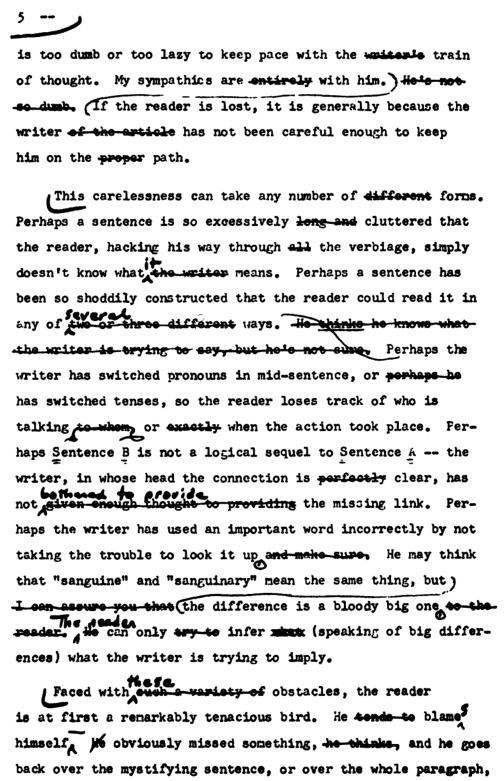
\includegraphics[width=0.9\textwidth]{figure/fig1-1.png}
\end{figure}


\begin{figure}[!htb]
\centering
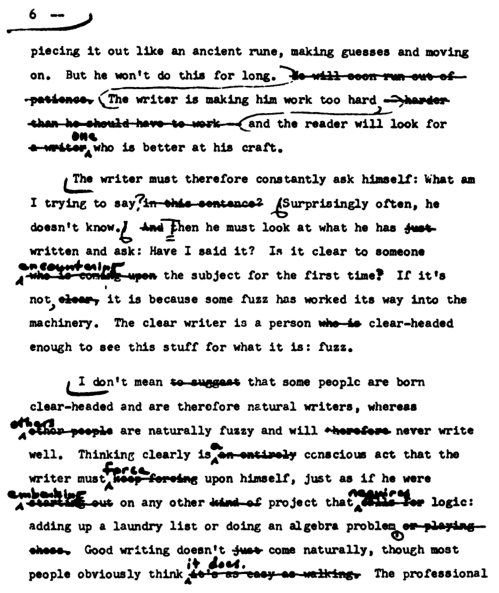
\includegraphics[width=0.9\textwidth]{figure/fig1-2.png}
\end{figure}


以上是《写作法宝》第一版本章终稿的两页。虽然这两页看起来像第一稿,其实已经修改和重新打过四五遍了——几乎每隔一页都是如此。每次修改我都尽力使所写的文字更紧凑、有力、精确,剔除所有无用的部分。然后再过一遍,朗读一遍,每次都惊讶地发现仍有许多赘词可以去除。(在后几版中,我去除了用来表示“作者”与“读者”的性别歧视性代词“他”。)
\chapter{激励工具}
上一章我们批驳了一系列“貌似有理”的不写作的理由,传递的信息是清楚的:根据计划来安排写作。计划表造就了高效的写作者,这是他们为什么能写出那么多作品的原因。不过有可能你在计划的写作时间里无所事事:你坐下来,泡上咖啡,打开电脑,却不知道要写点什么。改过自新的突击写作者通常都不懂如何管理他们的写作时间。因为他们以往的激励工具是“最后期限”和“罪恶感”,他们没有规划目标、同时管理多个写作任务和执行计划的经验。本章将介绍一些常见的能够提升你的写作动机和提高写作成效的激励工具。这些工具起作用的前提是你已经在按照计划表行事。如果你还没有这样做,那你尽可以固执地继续你临时突击的节奏。

\section{制定目标}
和商人一样,学者也喜欢讨论目标。有些学者非常痴迷于目标、举措和战略计划,所以他们成了院长或教务长。目标值得我们好好关注。清晰的目标本身就是直接的激励——它们能够帮助人们制订计划,采取有效行动并因为目标达成而感到自豪(Bandura, 1997)。没有清晰的计划,人们的行动是散漫而毫无方向的(Lewin, 1935)。为了能够写得更多,你需要明确写作目标。这个并不像听上去那样容易,计划常常因为目标设定不当而跑偏方向。设定正确的目标可帮助你成为一个高效的写作者。

那么你该怎样设定目标呢?首先要意识到目标设定是写作过程的一个环节。花上一个写作时间段来好好理清你的写作目标是个不错的主意,我通常一个月整理一次。计划是写作的一部分,所以计划多的人写得也多。第二步是把你的目标逐条列出来——这些目标是具体的需要完成的写作任务。例如修改和重新提交论文,开始写一篇新的文章,接受邀请为某一本合集写一个章节,把你去年写了一半的那篇论文重新捡起来,写一篇课题经费申请报告,或是写一本书。

你想写些什么?当悔过的突击写作者首次设定目标时,通常只有一个任务——是过去三个月以来他们心头一直在回避的那个恐怖的任务。当然要把这个列出来,但是不能仅此而已。在未来的几个月里,你还有什么其他想写的呢?是否在看得见的将来就有一个课题申请要截止了?在你的文件柜里是否有一个还没有发表的实验数据值得你再好好琢磨一下?是否有一篇一直想写而未写的评论文章?把这本书暂时放下,找些纸来,天马行空地列一些你想写的东西。

你决定了要写些什么以后——也许这张单子看起来很长——现在你需要把这些目标写下来。在你的写作过程中不断更新这份东西是浪费时间,所以找一块白板或者公告板,放在你的写字台旁边,然后骄傲地把你的目标一一列在上面。一个突击写作者在这么长的计划面前会感到非常焦虑,但是你有时间表啊!你会自问 “我能完成吗?”自律性强的写作者会大致想一想要花几个星期来完成单子上列的这些内容。在这个单子上划去一项任务是非常令人开心的。你可以贴个笑脸在上面,如果这是你的风格的话。

第三步是把每天要写的目标尽可能具体化。当你真的坐下来为了你的目标奋斗的时候,你需要把这些目标变成一个个小的目标。 “修改这篇论文”是一个写作任务,但是对于决定要写些什么而言,这个表述过于宽泛了。每当你开始工作的时候,都需要花一点时间想一下当天你想完成些什么。“写论文”这样的目标太宽泛了,你需要具体的目标。这里列举一些具体目标的范例:
\begin{itemize}
  \item 至少写200个字;
  \item 把昨天写的草稿打印出来,阅读和修改;
  \item 制订新的写作目标并把它们写在白板上;
  \item 把总论部分的前三段写好;
  \item 补充所有参考文献,然后把引文和参考文献梳理清楚;
  \item 重读津泽(Zinsser, 2001)的书的第二十二章和第二十四章,给自己充充电;
  \item 继续把昨天的“设定目标”部分写完;
  \item 头脑风暴,然后把新论文的大纲写好;
  \item 重读评审人的评论并把要修改的部分一一列出;
  \item 校对清样并寄出。
\end{itemize}

有些人对在目标里列出字数和段落数感到很吃惊。记住,这些是具体的目标。要着手完成一个宽泛的目如——如“修改和重新提交这篇论文”——是很难的,但是要理解“至少写200个字”很容易——你坐下来,打字。精力旺盛的安东尼·特罗洛普(Anthony Trollope)写作的时候会戴一块手表,他的具体目标是15分钟写250个字(Trollope, 1883/1999)。一定要养成制订具体、集中、详细的写作目标的习惯,这样能够避免不知道做什么和不知道怎么做。


\section{挑选优先项}
现在,你手里有一张写作任务的清单了 。在所有这些任务里,你应该先做什么呢?我问了身边的写作高手们是怎样挑选优先项的。下面是综合我自己和身边高手的经验后给出的一些参考意见。你可以以此为参考,并挑选自己的优先项,把它们写在你的写作任务清单旁边。

{\kaishu 1.校对清样和复审论文}

这一项几乎是所有人的首选。道理很简单,校对清样是论文发表前的最后一步了,而且与其他很多学术写作任务不同,这一项通常有严格的时间节点。出版商们往往需要你快速地校对和复审,通常在48小时内完成。在经历了数月或数年的数据收集和写作过程之后.你为什么还会拖延自己的论文发表呢?快快完成吧。

{\kaishu 2.完成有截止期限的任务}

大多数的写作任务都没有截止期限,所以那些有截止期限的任务都应该在计划表中占有优先位置。有截止期限的任务可能包括受邀写作的部分章节、课题申请报告或是行政报告。有些期限很死——大多数的经费提供机构都过期不候,而有一些期限则比较灵活。就我个人而言,我并不把这一项列为我的优先选项,原因是我已经不像过去那样死抠截止期限了。如果你很好地执行了写作计划,那么你总是能够提前完成。截止期限对突击写作者来说是最大的激励,对于一个严格自律、有良好计划的写作者来说则没有什么用。

{\kaishu 3.修改论文以重新提交}

大多数的论文都会被拒。如果你有幸收到修改并重新提交的通知,千万别浪费了。重新修改后的论文比新提交的论文发表的几率高,所以你应把这一项列为优先项。

{\kaishu 4.评审稿件或课题申请报告}

这一项颇受争议。我的同事们就审稿是否应该被列为优先项有不同的意见。有些人认为这一项属于优先“非写作”项,应该快速完成,但不是用写作时间去完成。有些人对评审论文不怎么感冒,常常放在一边。不过我个人觉得这是一项颇为重要的工作,把它放在比较重要的位置。同行评审的过程与评审人关系甚大。心理学界的审稿流程之慢,已经影响到这个领域的发展。如果每个人都看得快一些,那么每个人也会写得欢快一些。快速地完成评论也有助于和编辑们建立良好的关系,因为他们总是对速度过慢的审稿人意见颇多。对于课题申请报告也是一样:课题评审对申请者而言事关重大,所以还是早点把它们做完为好。

{\kaishu 5.开始写作新的论文}

每一篇发表的论文都是从一份草稿起步的。从头写一篇新的论文对于突击写作者来说很难:他们常常花了几个月才开头,他们也是心血来潮时才做文献综述和数据分析部分的。其实,如果你能照着计划来,写一篇新的文章是相对容易的(与撰写课题申请报告、著作和修改论文相比)。第六章将就实证研究型论文写作给出一些建议。

{\kaishu 6.写各种杂文}

对所有不太重要但是仍然需要完成的写作任务,我们姑且称之为杂文。例如写一篇通讯短文。这能够帮助你暂时从那些主要的写作任务中解脱出来,捣鼓捣鼓些小玩意,获得片刻的安宁和乐趣。

几乎所有我调查的对象都提到,他们会把有研究生参与的写作任务放在特别优先的位置。比如,他们通常会花时间修改一篇要重新提交的论文,但是,如果要写一篇新论文,而这篇论文是与某个研究生合著的,他们会把它放在更为优先的位置。这是明智的建议。我也常常把优先权给那些我不参与实际写作的合著论文。试想一下,你辛辛苦苦地写了草稿,发给第二和第三作者征求修改意见,但是从来得不到反馈,这会是什么感觉?被合著者拖累是令人抓狂的,尤其是当这个合著者还不负责具体写作的时候。突击写作不是一个好习惯,而与人合著时还拖延则更加糟糕。

研究生应该和教授们有着不同的写作优先项。以下清单是我在采访了一些优秀研究生或是刚刚毕业的学生后整理的。

{\kaishu 1.有截止期限的写作任务}

研究生学习期间会有很多有截止期限的写作任务,例如某门课程的作业。很多学生抱怨他们的课程作业占用了太多写作时间,使得他们无法花更多的时间完成更为重要的写作任务,例如硕士论文。这是事实,但是截止期限就是截止期限,而这些小的作业或论文对未来的学术生涯未尝不是一种有益的尝试。如果你需要更多的时间写作,那只能在你的写作计划表里安排更长的时间。经费申请报告——例如研究生奖学金的申请——也同样有截止期限,而且它们非常重要,应该努力尽快完成。

{\kaishu 2.与学位授予相关的写作任务}

研究生学习期间,你需要写很多与学位授予相关的文章,例如硕士学位论文、综合考核报告、资格论文和博士学位论文。这些要想毕业就必须完成的东西最好快点写完。上述这些任务的成果有时候还能转化为可发表的论文,所以很多学生都会把与学位授予相关的论文与真正的专业写作结合起来。

{\kaishu 3.公开发表的专业论文}

科学研究只有在它公开发表,使之得以为同行所阅读和评论之后才能实现其真正的价值。你完成了论文,院系委员会也觉得你干得不错,但这是不够的,只有论文公开发表后学术界的其他同仁才能有机会更仔细地研究你的论文并认识它的价值。优秀的硕士学位论文或博士学位论文应该寄给专业的期刊。此外,你还应该力求在硕士学位论文和博士学位论文以外发表更多的专业论文。你要抓住每一个机会参与研究和专业写作。如果你很好地对写作加以规划,你将是你们项目里最高产的研究生。

{\kaishu 4.其他}

研究生常常写许多五花八门的文章,比如书评或报刊杂文。和其他类型的写作一样,写这一类的文章也是很好的锻炼,也很有意义。不过与专业水准的、存档留案的论文(比如期刊论文或专著的某个章节)比起来,这些杂文就显得不那么重要了。如果要在两个中间作出选择,那就应该把专业写作放在前面。

当我们在讨论选择优先项的时候,总有人会问:“那万一我觉得没什么可写呢?”对教授们来说,极少会感到没东西可写。恰恰相反,大多数我认识的教授都有堆积如山的未发表的数据。收集数据的过程是简单的,写作是困难的。如果你有一些十年前就已完成的实验却从未发表过,那我肯定你需要一段时间才会感到没有东西可写。更何况,写作促进写作。正如博伊斯(Boice, 1990)所发现的,那些定期写作的人会比那些只在灵感来临时写作的人有更多的创见(参见第二章)如果你觉得没有东西可写,那还是花一段写作时间来重新列一下你的写作目标吧。

然而,研究生们或许的确会觉得没有一个现在要跟进的写作任务。也许你刚刚完成了你的论文,暂时没有其他任务;也许你刚刚入学不久。别害怕,这个时候你有两个选择。首先,你可以参与一项正在进行的写作任务。你的导师,跟其他大多数的教授一样,或许正在为一大堆写作任务而头疼。敲开他/她的办公室然后说:“我最近看了一些关于如何成为更好的写作者的书,其中一本建议我敲开您的办公室,然后问问我是否能参与到一些写作任务中来。如果您有一些论文要写或是有一些数据要整理,我愿意帮忙。”很有可能你的导师会大倒苦水。教授们都希望自己的研究生在专业研究和写作方面倍加勤奋,所以你的导师一定会为你想加入而感到高兴。

另一个解决没有东西可写的办法是,你可以用写作时间来做些对专业发展有益的事。我读研究生时得到的最好的建议就是,“总是让自己不断思考”。研究生院是疯狂的,当你在为一大堆截止期限埋头奋斗的时候,你往往会忘了自己的长期目标。每周给自己留些固定时间,就能够利用它们来读些关于写作和教学的书,回顾自己的研究,想想你的职业规划。


\section{监控进展}
大多数人都不清楚自己究竟写了多少东西,是多是少。因为他们总是带着某种沾沾自喜、自我安慰的态度来审视自己,大多数人都认为自己比实际上要来得高效。为了写得更多,你必须带着某种冷峻、客观的态度来监控你的写作进展。有关自我管理的研究表明,仅仅设定目标和选定优先项是不够的:人们必须就达到目标的进程进行监控(Carver \& Scheier, 1998; Duval \& Silvia, 2001)。

监控写作进展有很多激励作用。首先,时时直面你的目标能够加深印象,防止你淡忘。许多人对如何管理他们写的东西很不在行。监控进展能够帮助你关注你正在进行的任务。其次,监控本身也足以帮助你坐下来开始写作。行为研究表明,自我观察本身就能够促进期待行为的发生(Korotitsch \& Nelson-Gray, 1999)。例如,想要存钱的人应该记录他们每天的花销,因为记录他们每天花了多少钱能够让他们节省开支。同理,想要定期写作的人应该追踪他们是否定期坐下来写作了:你放弃了某段写作时间,所以不得不在一个Excel表格里打上一个大大的“零”的时候,你会很奇怪地感到某种鞭策。最后,监控你的写作能够帮助你制订更合理的目标。经过一段时间,你将能积累足够的资料来合理地判断你大概需要多久来完成某项写作任务。制订更合理的目标,反过来又能够保障更高效的写作。

高产的写作者通常都会做这样或那样的监控。方法有很多种。在这部分里,我想介绍一下我的方法。每次我向别人介绍我的方法的时候,他们都给我一个诧异的表情,就好像听说我要拿伯尔尼山犬的毛来做被子似的。我用的系统看起来又蠢笨又牵强,还有点奇怪,不过它的确能帮助我集中精力。我有一个文件名是“写作进程.sav”的SPSS文件,图3.1是它的截图。我记录月份、日期、星期和年份。这些变量帮助我定位某一个日期。统计项是字数、目标和任务。在字数一栏,我键入每天我写的字数。字数统计工具能够轻松地告诉我文章的字数;每天开始和结束写作的时候都统计一下就能清晰地显示出一天的成果。你会注意到字数这一栏有很多空白。我之前已经强调过了,写作包含很多任务,不仅仅是码字。有时候我读些论文,有时候我填写课题申请表,有时候我重读需要修改并重新提交的论文。这些日子的字数一栏就会是空白的。设置目标一栏的目的就是回顾我是否完成了当天的目标。我个人的目标很简单,坐下来做些有利于推进研究的事,所以我会把这个变量记为\{0=未完成,1=完成\}。图3.1所示的那段时间我干得不错;只有7月5日那天我未完成我的既定目标,其他日子我都完成了。任务一栏用来描述我当天的任务。如实记录任务能够让你更清楚地知道你要花多少时间来完成一项任务。有时候会觉得某个任务没完没了,但是有可能它比你记忆中的已经简化了而你没有发觉。

\begin{figure}[!htb]
\label{fig3-1}
\centering
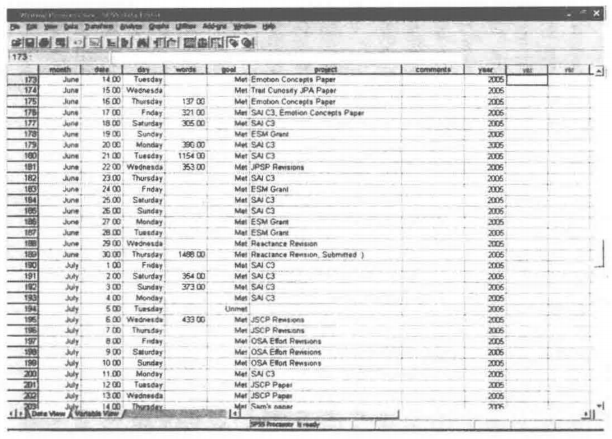
\includegraphics[width=0.9\textwidth]{fig3-1.png}
\caption{我用“写作进程.sav”文件来监控自己的写作进程}
\end{figure}

那些还死抱着各种无力借口的突击写作者可能会说“但是我不会用SPSS”或者“可是我只用SAS”!其实任何统计软件或者制表软件都可以做这件事,实在不行,画好线的笔记本和铅笔总是有的。监控本身才是关键,技术问题不是问题。不过,统计软件能够让你深入挖掘你的写作数据。如果你是一个统计控——这年头又有谁不是呢——那么你会爱上获得你的写作数据的感觉。我写了一个简单的SPSS公式来计算一些可见的数据和柱状图。当我开始写一篇新的文章时,我平均每天写789个字,如图3.2所示。听起来不是很多,不过字数逐日增加。图3.3显示的是每个月的目标完成情况。根据数据,在过去的12个月里,我在计划写作的日子中有97\%的日子实际坐下来写作了。我不是完美的,不过我对这个数据还是满意的。监控是为了改进,如果有一天这个数据达到100\%,我会感到非常骄傲。如果你很好奇,你还可以把目标达成情况和字数都按照天数来统计。所以,如果有人问我能写多少,我会回答97\%的工作日我都在写作,且每天我平均写789个字。他们可能会给我一个“伯尔尼山犬毛被子”的面孔,但这无所谓。

\begin{figure}[!htb]
\label{fig3-2}
\centering
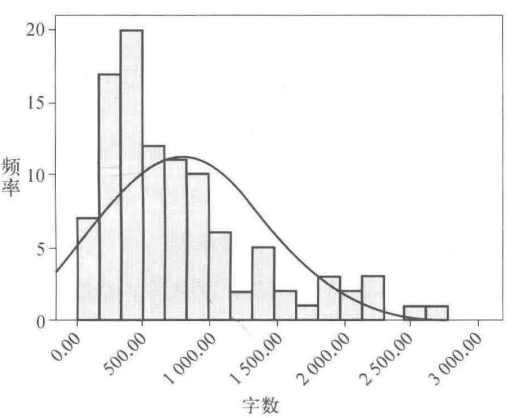
\includegraphics[width=0.9\textwidth]{fig3-2.png}
\caption{过去12个月每天的平均写作字数}
\end{figure}


\begin{figure}[!htb]
\label{fig3-3}
\centering
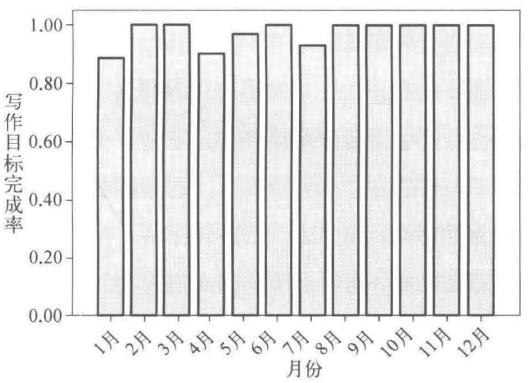
\includegraphics[width=0.9\textwidth]{fig3-3.png}
\caption{过去12个月每月的写作目标完成率}
\end{figure}


当你完成一项写作任务时,别忘了奖励自己。自我强化和依随性管理被证实对培养好习惯有很大的帮助(Skinner, 1987)。当你提交了一篇论文或是一份课题经费申请报告,给自己买杯好咖啡或是吃一顿奢侈的午餐,或者买一张古老的好莱坞-维克菲尔德式的书桌。写作的回报往往是滞后的——通常都要等上好几个月才能有杂志编辑或者经费评审委员会的消息——所以即时的自我奖励能够帮助你维持兴趣。不过,只有傻瓜才会以偷懒不写作的方式来奖励自己。永远不要以不写作的方式作为对写得好的奖励,以抛弃你的写作时间作为奖励,就好比以抽一支烟来奖励你戒烟成功。写作计划的有效执行有赖于超强的习惯掌控力:不要丢掉好的写作习惯。


\section{文思枯竭}
“等一下,”你也许会说,“到目前为止,这本书还没有提到任何关于文思枯竭的问题。当然啦,你可以制订计划,设定目标,然后监控进展,然而如果你实在写不出来怎么办?”我非常喜欢“文思枯竭”,这与我喜欢树精或是会说话的林中动物的道理是一样的——它们都很令人着迷,而且它们都不存在。当人们跟我说他们有时候真的会文思枯竭,我总是问他们,“你们到底要写什么?”学术写作者是不可能文思枯竭的。千万不要把自己和那些在艺术系教创作的朋友混为一谈。你又不是在创作一个长篇故事或是在写一个直指内心深处某个神秘角落的深刻隐喻。你对方差的精妙分析不会让读者们感动落泪,倒是有可能枯燥得让人掉眼泪。人们也不会影印你的参考文献目录并发给朋友们,期待能够给他们带去灵感与启迪。小说家和诗人是充满诗情画意的风景画家和肖像画家;学术写作者则是手握大型喷漆器重新粉刷地下室的油漆工。

文思枯竭是一个典型的倾向性谬论:对行为的描述同时被用来解释被描述的行为本身。所谓文思枯竭,说白了就是什么都没写。你说自己文思枯竭了,所以写不出东西,就相当于你说自己写不出东西是因为你什么都没写。这样的说法毫无意义可言。治疗文思枯竭的办法——如果你可以治愈无病呻吟——就是写作本身。建议重读第二章博伊斯(Boice, 1990)的实验。那个研究表明,苦苦挣扎的写作者们只要按照计划不断写作,就能写出很多东西——就这么简单。相反,那些非要等待“灵感”的人几乎什么也写不出。如果你真的文思枯竭,你有三个选择:(1)放下你手上正在摆弄的诗集,重新回到你的期刊论文写作中;(2)说服树精或会说话的动物们帮你写问题讨论部分;(3)重新制订你的写作计划,然后重新执行它。

就好像外星人只绑架相信存在外星人绑架事件的人一样,文思枯竭只会发生在相信有文思枯竭这回事的人身上。写作计划——这是个很神奇的东西——最神秘的部分就是,有计划的作者不会感到文思枯竭,不管到底有没有这回事。高效的写作者无论想不想写,都会按时写作。有时候他们写得不多——写作是件艰难的事情,但是不管怎样,他们都会坐下来写,不为那些虚无缥缈的事情所干扰。

\section{小结}
本章介绍了一些能够帮助你成为一个更高产的写作者的激励措施。制订好写作计划表以后,你需要确定写作目标并把它们写下来。然后,在你坐下来写作以前,先花一分钟想一想你今天想干什么。选定优先项能够马上帮助你摆脱同时进行多个写作任务的压力。监控你的写作能够让你集中精力完成目标,监督你不要放弃任何一天,告诉你你能写得多好,还能提供足够的数据让那些怀疑你的突击写作者闭嘴。任何能把本章提到的建议都一一做到的人,毫无疑问都能写得很多。
\chapter{风格}
作者努力写出简洁的句子,但总有那肿胀的怪物埋伏在暗处捣乱。有关写作初期的告诫就谈到此。

“但是,”你也许会说,“如果我去除你认为是赘语的所有部分,如果我将每一句话都剥到只剩骨头,那我还能剩下什么?”这个问题问得合理。简洁推到极致也可能会指向一种不比“狄克喜欢珍妮”和“看斯波特跑”这样的句子更复杂多少的风格。

我将首先从木匠手艺的层面回答这个问题。然后涉及更大的问题,即作者是谁,如何保护作者的身份。

很少有人意识到自己写得多么糟糕。没人向他们指出有多少过剩或含糊的词语溜进自己的写作风格中,以及它们如何阻碍了作者想说的话。假如你给我一篇八页的文章,我叫你删减到四页,你会叫喊说那做不到。然后你回家去做,结果会好得多。之后便是难的部分:删减到三页。

要点是你必须先将自己的写作拆开,然后再搭建起来。你必须知道基本工具是什么,以及其预设的作用是什么。再拿那个木匠手艺比喻为列,首先必须锯好木头,然后钉钉子。之后,你如果有雅兴,再切修棱角、添加别致的顶部。但千万不要忘记你是在练习一项基于一定原则之下的技能。如果钉子不牢,房子就会坍塌。如果动词不牢、句子结构摇晃,句子就会分崩离析。

我得承认,有一些非虚构作家,如汤姆·沃尔夫和诺曼·梅勒,他们建构起了不起的房屋。但这些作家花了许多年来学习技艺,最终才搭建起神奇的塔楼和空中花园,使我们这些从未梦想过如此装饰的人惊叹不已。他们知道自己在做什么。没人一夜间就成为汤姆·沃尔夫,就连他本人也不能。

那么首先要学会钉钉子。如果你所建房屋既结实又好用,就该对具简洁之力感到满意。

但你没有耐心去成就一种“风格”——去修饰简朴的词语,这样读者就会把你认作一种特殊的人。你只会寻觅花哨的比喻、华而不实的形容词,就好像“风格”是什么能在风格店买到的东西,是可以用装饰漆那鲜亮的颜色装饰词语的东西。(装饰漆是装修工用的彩色漆。)风格店并不存在,风格对于写作中的人是有机体,就像头发是他自己身体的一部分,或者假如他秃顶,那么就是他身体缺乏的那部分。试图添加风格就像加假发在秃头上。瞧第一眼时,之前秃顶的人看起来年轻,甚至还帅气,但瞧第二眼时——看假发时人们总会瞧第二眼——那人看起来就不对劲了。这里的问题并非是他看起来没有梳理好,他梳理得很好,我们真得敬佩假发匠人的高超工艺,问题是他看起来不像自己了。

这个问题是那些特意装点自己文体的作家的通病。你丧失的是使你自己独一无二之处。读者会看出你是否在装腔作势。读者要的是,与他们交谈之人听起来是真挚的。因此,写作的一个基本准则是:做你自己。

然而,没有什么准则比这一条更难遵循。这要求作者做到两件事,而按其新陈代谢的本能来说,这些都是难以做到的。他们必须放松,必须有信心。

叫作者放松就像在检查疝气时叫人放松一样;至于信心,看,他多么僵硬地坐着,眼睛直勾勾地盯着等待他造词儿的电脑屏幕。看,他多么频繁地站起来找吃的或喝的。作者会想方设法躲避写作实践。我可以证明我在报社工作期间,作为记者,我每小时去饮水机的次数大大超过身体对水的需求。

如何拯救作者出苦海呢?很不幸,并没有拯救的办法。我只能安慰大家说并非只有你的遭遇如此。有些日子好过一些,另一些日子则难熬到让你绝望,不再想写作。大家都有过这些日子,而且还会有更多这样的日子。

当然,最好还是尽量减少难熬的日子。这就使我回到如何放松这个问题上来。

假如你就是那位坐下来准备写作的作者。你想到你写的文章必须具有一定的长度,不然就不会显得重要。你想到文章印出来有多么庄严。你想到那么多人阅读你的文章。你想到文章必须具有重重的权威性。你想到文章的风格必须炫目。怪不得你会浑身发紧:你在忙于想着自己甚至还未开始的文章写完之后所要承担的巨大责任。而你发誓要对这一任务称职,于是四处找大词,找那些如果你不是想刻意给人突出印象就根本想不到的词,并且一头栽进去。

第一段是一场灾难——整段话成了似乎来自机器的一系列笼统词语的组合。人是不会那样写的。第二段也好不了多少。但是第三段开始有点儿人情味,而到了第四段你开始听起来像自己了。你开始放松了。令人称奇的是,编辑会常常删掉文章的前三四段,甚至前几页,而始于作者听起来开始像自己的部分。前几段的问题不只是缺乏人情味和浮夸华丽,而是根本就没说什么,只是刻意地要写出一个花哨的前言。作为编辑,我总是在寻找说类似以下这样话的句子:“我永远不会忘记那一天……”这时我就想,“啊哈!真人说话啦!”

作者用第一人称写作显然是最自然的。写作是把两个人之间密切的交往付诸笔端,写作保持人情味才会顺畅。因此我敦促人们用第一人称写作,用“我”或“我们”。但大家表示抗拒。

“说我认为什么,或者我感觉什么,那个我是谁啊?”他们问。

“不说你认为什么,那么你又是谁呢?”我回答他们,“只有一个你。没有任何其他人想的和感觉的一模一样。”

“可是没人会在乎我的观点,”他们说,“那样会让我觉得太突出了。”

“如果你对他们讲述有趣的事,他们会在乎的,”我说,“而且要用自然而然的词语讲述。”

然而,要作者用“我”并不容易。他们认为必须先赢得袒露自己情感和思想的权利,不然就会显得自以为是,或者不庄重。此类恐惧也影响了学术界,因而出现了学术性的“某人/有人”的用法(“有人不能苟同于莫尔特比博士对于人类状况的观点”),或者无人称的用法(“希望费尔特教授的专著会理所当然地拥有更广泛的读者”)。我可不想见用“有人/某人”这样的人——很乏味。我要的是对自己的话题有激情的教授来向我诉说该话题为何使他着迷。

我意识到写作中有广大领域不允许用“我”。报纸不要第一人称代词“我”用于新闻报道中;许多杂志也不要它出现在文章中;商业、社会机构不要它用在大量发送到美国家庭的报告中;大学不让把“我”用在学期论文或学位论文中;还有英语教师也不赞成用第一人称代词,除非是作为书面语的“我们”(“我们在麦尔维尔对于白鲸的象征用法中看到……”)。以上那些禁用是合理的。报纸文章就应该由客观报道的新闻构成。在学生没经过一番挣扎学会从其内在优点和外在评论评价一部作品之前,教师不希望学生避重就轻地发表意见——“我觉得哈姆雷特挺愚蠢”。我也理解教师的这些想法。“我”这个词有可能变成某种自我陶醉和自我逃避的工具。

然而,我们的社会已经变得害怕袒露自己的心声。向我们发送宣传品、寻求支持的社会机构听起来惊人地相似,但所有这些机构——医院、学校、图书馆、博物馆、动物园等——当然是由那些有不同梦想和展望的男男女女创建和管理的。这些人都在哪儿?在所有那些非人称的被动语态句子中,如“已经采取行动”和“重点已经确定”,很难瞧见他们的真面目。

即使是在不允许用“我”的时候,也有可能传达一种个性化的我的意思。政治专栏作家詹姆斯·赖斯顿在专栏写作中并没用“我”,但我却很清楚他是什么样的人,对其他很多随笔作家和记者,我也可以这么说。好作家在字里行间是看得见的。如果不允许你用“我”,写作时至少要用“我”思考,或者第一稿用第一人称写,然后再把“我”去掉。这样能预热你的非人称风格。

风格与心理绑在一起,写作的心理机制根深蒂固。我们表达自己的特有方式,或由于“作者心理阻滞”而没能表达好自己的原因,部分埋藏于潜意识心理中。作者心理阻滞的种类就像作家种类一样多,我也没有捋清它们的意图。这是一本薄书,我的名字也不叫西格蒙德·弗洛伊德。

但是我也注意到避免“我”的新理由:美国人在言辞上不愿意冒任何风险。我们的上一辈领袖们直言不讳自己的立场和信仰,现今的领袖们却千方百计地巧用词语逃避这一宿命。看看他们如何在电视采访中拐弯抹角,就是不立场鲜明。我记得有一次福特总统向一行来访的商人保证他的财政政策会奏效。他说:“每月我们所看见的是不断增亮的云彩,此外别无他物。”我对此的理解是那云彩还相当黑。福特的句子含义模糊不清,等于什么也没说,却给他的选民打了镇静剂。

后来的当局者们也并没有起色。国防部长卡斯帕·温伯格在1984年评价波兰危机时说:“有继续严重关注的余地,而且形势仍然严重。严重的形势持续越长,严重关注的余地也就越多。”老布什总统被问及他有关突击步枪问题的立场时说:“有不同的群体认为可以禁止某种枪支。我不在其列。我是在那些深刻关注者之列。”

不过我的全能冠军当属70年代身为四任主要内阁成员的艾略特·理查森。很难确定从他那模棱两可的句子宝库中选哪一句,还是看这句吧:“但是呢,均衡地来讲,我认为少数族裔及妇女维权行动还是取得了一定的成果。”\footnote{原文如下: And yet, on balance, affirmative action has, I think, been a qualified success.}一句13个单词的话中就有5个词含义模糊。在现代公共话语中,我给它最空泛句子一等奖,但与其媲美的还有他分析如何消除生产线工人单调乏味的句子: “这样呢,最后,我形成一个坚定的信念,我在开始提到过:就是这个问题太新,无法最终判断。”


那就是坚定的信念吗?像摇摇晃晃来回摆动的年迈拳击手这样的领袖不能鼓舞信心——也不配鼓舞信心。作家也是如此。推销你自己,你的题材就会发挥自己的吸引力。相信自我身份,相信自己的见解。写作是一种自我行为,你得承认这一点。要全力以赴使自己不断向前。
\chapter{简洁、单刀直入的文风}
学术期刊散发着垃圾写作的酸腐味——我总是把期刊放在离书桌最远的书架上,以免被熏到。但是如果你有机会与这些文章的作者面对面交流,你会发现他们对自己的研究津津乐道,他们的口头表达是那样清晰、生动和有趣。哪里出了问题?尽管这本书的主题是写得更多,而不是写得更好,但你还是应该花点时间来掌握一些要领,让你的作品更有力度。如果人们坚持执行写作计划,大概一个星期以后他们就能写得更多,要写得更好则需要更长的时间来学习——所以我们应该从现在就开始。本章将介绍几个能够帮助你提高写作水平的小技巧。

\section{诊断问题}
有三个原因会导致写作水平偏低。首先,学者们喜欢显摆聪明。有一则德国格言说:“水面颜色深的湖必是深湖”所以,学者们常常弃好词而不用。比如,他们不用“聪明的”(smart),却用“老练的”(sophisticated)或“渊博的”(erudite)。我应该这样说,“水体的透明度的最小值往往与水的深度之间有着极高的相关性(p<0.05)”。其次,学者们从未学过好好写作。他们在研究生院的导师可能不是一个好榜样,而他们引以为榜样的期刊文章也散发着酸腐的垃圾味。最后,大多数学者都没有花足够的时间来成为一名优秀的写作者。和其他所有的技能一样,写作技能也需要长时间的勤学苦练(Ericsson, Krampe \& Tesch-Romer, 1993)。人们必须学习好的写作规则,然后花大量的时间来练习。

为了解决第一个问题,你必须修正对学术写作的态度。也许有些读者会因为你写的东西晦涩难懂而觉得你很聪明,但是你并不需要这样毫无眼光的读者。大多数的科学家都会被好的观点和有趣的发现吸引,所以不要把你的意见藏在一大堆垃圾英语背后。为了解决第二个问题,仔细地阅读这一章,然后买一些其他关于写作的书来读。本书“推荐阅读:那些关于写作的好书”部分附有关于文风和语法的参考书目,或许对你有所帮助。为了解决第三个问题,你需要阅读上述书籍,并在写作时多加练习。要不了多久,你就会逐渐形成独具一格的文字风格,而不再是那个让人不知所云的无名氏了。

\section{选择“好词”}
写作的核心在于用好词。为了写得好,你必须选择“好词(good words)”。英语中包含很多词,其中有很多简短、有表现力而且常见的词——要选用这些词。避免用那些听起来很深奥的时髦词组,更不要用那些学术腔太重的词。除了帮你提高写作水平,选择“好词”也是对读者的一种尊重,因为对他们来说,英语可能是他们的第二、第三或者第四语言。外国学者常常在阅读文章的时候备有双语词典,如果你选的词不在词典里,他们就理解不了。他们会怪自己误解了你的意思,其实你才是应该被责备的人,因为你没有顾及他们的实际情况。

“那专业词汇呢?”你也许会问,“我怎么可以不用‘刺激呈现的异步性(stimulus onset asynchrony)’来写一篇关于刺激呈现的异步性的文章?”科学在需要的时候会创造出新的词——这些专业词汇是有用的。如果用常用的词来解释,这些专业词汇是很容易被理解的。我们应该保留科学词汇,剔除那些从商学、市场学、政治学和军事学那里借用来的词汇。我们不需要诸如“物质激励(incentivize)”或“瞄准(target)”之类的动词,也只有玻璃清洗工才需要“透明(transparent)”之类的形容词。为了连贯,请重复使用同样的专业词汇。不断变换的心理学专业概念会把你的读者搞晕:

{\kaishu 前:神经过敏症指标高的人比体验厌恶情感状态倾向指标低的人反应慢。

Before: People high in neuroticism responded slower than people low in the tendency to experience aversive affective states.

后:神经过敏症指标高的人比神经过敏症指标低的人反应慢。

After: People high in neuroticism responded slower than people low in neuroticism.}

而且有些专业词汇真的是糟糕透顶,所以不要不假思索地引用你在专业期刊上看到的词汇。发展心理学家对“道(path)”和“路(way)”都不满意,他们喜欢用“路径(pathway)”;在某些吹嘘的场合,“路径”变成了“轨道(trajectories)”。认知心理学家喜欢“澄清(clarify)”什么是“消除歧义(disambiguate)”。临床心理学家喜欢说病人“呈现(present)”出某种症状,感觉对方好像是一个情绪低落的管家,托着一个盛满“负面情绪”或“低质量睡眠”的大盘子。临床医生也不再用“医嘱(manual)”和“遵医嘱(follow manual)”,他们发明了“医疗干预(manualized interventions)”一词。情感心理学家生怕他们的读者不理解“评价(appraisal)”这个词的意义,他们喜欢说“认知评价(cognitive appraisal)”“主体评价(subjective appraisal)”有些人还是怕别人不理解,索性说“主体认知评价(subjective cognitive appraisal)”。做跨学科研究的心理学家提出了“生物——社会”模型(biosocial models)、“社会——心理”模型(psychosocial models),最近又有了“生物——心理——社会精神”模型(biopsychosocialspiritual models),用以取代原有的狭隘的“生物——心理——社会”模型(biopsychosocial models)。

心理学家特别青眯“坏词(bad words)”,不过他们不说“坏(bad)”,而是代之以“deficient(有缺点的)”或是“suboptimal(非最理想的)”。心理学家喜欢用“现有文献(existing literature)”, 难道我还需要阅读和引用“不存在的文献(nonexistent literature)”吗?任何在读文献的心理学家都应该知道我们这些专业期刊就是这样“可怕而真实”。“现存文献(extant literature)”是同一宗罪的升级版。那些写某两样东西之间“失联(disconnect)”的心理学家恐怕是与他们的字典“失联”了,因为他们本可以在字典里找到无数更好的词,如“差异(difference)”“区别(distinction)”“分离(seperation)”和“差距(gap)”。有些人在写某一关于某一问题的论文时,把“人”(a person)称为“个体”(individual)而把“人们”(people)称为“个体们”(individuals)。这些人忘记了“个体”是一个模糊的概念:试想,“我们观察一个个体\_\_\_\_ 。”画横线部分应该补充一个名词(例如:兔子)还是一个动词(例如:走路)?你在和朋友说话的时候从不说“个体”或“个体们”,那为什么在和广大的科学界同仁交流的时候要装腔作势地这么说呢?选个对的词,比如人(person)或人们(people)就可以了。而“persons”则更为可恨,这样的词大概只有小镇警长在寻找失踪人口时才会用到吧。

说到“人们(people)”,我在描述我的研究参与者时已经不再用“参与者(participants)”一词了。我的朋友们有研究鸟类、婴儿、老鼠或是学区的,他们的“参与者”和我的完全不同。我研究的是成年人,所以“人(person)”或“人们(people)”是对我的研究对象的准确界定。如果这个决定让你不安,别害怕——美国心理学会(APA)不像时尚界,这里没有“警察”。“参与者”是一个模糊的词,心理学家应该选择更确切的词。比方说,有些研究人员是从儿童、教师和家长那里收集资料来研究儿童心理学的,他们的参与者就应该是上述三个类别的人。不要觉得有什么不妥,就应该称他们为儿童、教师和家长。如果你研究老年人或是年轻人的认知过程,为什么不在你的研究方法和结论部分称他们为老年人或是年轻人?现在就把你的研究方法部分重新写一遍,把所有的“参与者”都改成更为确切的词,这样你会觉得舒服很多。

一些缩略词和首字母简称也是不妥的。我见过有些人把很常见的词,比如“焦虑”(anxiety)或“沮丧”(depression)缩写为ANX和DEP,把简单的词组,比如“引发焦虑”(anxious arousal)和“缺乏快乐感而沮丧”(anhedonic depression)简写成ANXAR和ANDEP, 然后兴奋地讨论ANX、ANDEP、DEP和ANXAR的区别。缩略词和首字母简称只在比它们代表的原词(或词组)更易于理解的情况下才有用。SES(社会经济地位)和ANOVA(方差分析)是好的缩写,ANX和DEP则不是。有些作者认为他们用简称代替常用词能够避免行文冗长。比如写一本关于如何写得更多的书,他们会想着把“写得更多”缩写为WAL。其实读者会觉得读这样的缩写比读原词更乏味。为了避免拐弯抹角,你应该少用缩略词。

删去诸如“非常(very)”“相当(quite)”“基本上(basically)”“实际上(actually)”“事实上(virtually)”“极端地(extremely)”“明显地(remarkably)”“完全地(completely)”“根本(at all)”之类的词。基本上,这些相当无用的词事实上毫无意义,它们事实上就像水草,实际上会完全地阻塞你的句子。在《垃圾英语》一书中,肯·史密斯(Ken Smith, 2001: 98)把这些词称为“寄生强化剂”(parasitic intensifiers)。

{\kaishu 原本含义确切的词现在好像需要附加这些强化剂才能恢复原有的能量。现如今,表达观点或是反对的立场时非要加上“有价值的”或“坚决的”之类的词,否则就会显得不温不火。这些强化剂削弱了原意。}

如果你真心领会了斯特伦克和怀特(Strunk \& White, 2000: 23)关于“省略无用的词”的建议,但是又不太确定哪些是无用的词,那么上述这些“寄生强化剂”基本上就是应该完全删除的。


\section{写出有力度的句子}
现在你对遣词有所体会了——“我上篇文章有没有用‘个体’?”——那么是时候想想如何造句了。“每当你造句的时候,”谢里丹·贝克(Sheridan Baker, 1969: 27)这样写道,“应该就像呼吸一样自然,或许也同样缺少变化”。不断重复类似句型的作者,就好像在不断地使用复读机。英语有三种不同类型的句式:简单句、复合句和复杂句(Baker, 1969; Hale, 1999)。简单句只有一个主——谓结构。学者们对清晰的简单句不屑一顾。这实在可惜。复合句有两个从句,每个句子能够独立存在。有时候用关联词来连接非独立从句,有时候分号能起到同样的作用。与简单句和复合句不同,复杂句包括独立从句和非独立从句。复杂句如果用得好,能够使你的文章干净利落、张弛有度。

在自我感觉良好的时候,我相信并列句是为心理学家发明的。我们总是在写关系、对照和比较:外向型指标高的人和外向型指标低的人、控制组和实验组、时间段一发生的事情和时间段二发生的事情。好的写作者合理地运用并列句来描述关系;拙劣的写作者则尽量不使用并列句,因为他们觉得并列句很啰嗦,相反,他们通过变换词语和句式发明了很多别扭的句子。

{\kaishu 前:双任务组的人在一组“嘟嘟”声的引领下阅读一列词汇清单;另一个组的另外一些参与者仅阅读词汇而不会听到任何声音(“控制组”)。

后:双任务组的人在一组“嘟嘟”声的引领下阅读一列词汇清单;控制组的人仅阅读词汇清单。}

有些并列句式用“标准——变量”的格式:先描述共性,而后解释差异。

{\kaishu 更好:每个人都阅读一列词汇清单,双任务组的人在一组“嘟嘟”声的引领下阅读,而控制组的人仅阅读。

更好:每个人看一组20幅画。控制组的人只是看一看这些画,评估组的人则要标出对每幅画的喜爱程度。}

很多人根本不知道如何用分号——这个符号是并列句的最佳搭档,却常被忽略。就像人们不喜欢球迷或俱乐部的年册一样,很多作者从高中就养成的对分号的不信任绝对是一种偏见。我们要解决这个问题——我们要分号。分号必须连接独立从句;句子的任一部分必须能够独立存在。与句号不同,分号表示两句句子间的紧密关系。与逗号及随之出现的“和”也不同,分号表示两个部分间的平衡。分号是理想的连接两个并列句的工具:

{\kaishu 前:在时间段1, 人们阅读词汇。在时间段2,他们尝试记住尽可能多的词。

后:在时间段1, 人们阅读词汇;在时间段2,他们尝试记住尽可能多的词。

前:阅读组的人阅读词汇,听力组的人听这些词的朗读录音。

后:阅读组的人阅读词汇;听力组的人听这些词的朗读录音。}

除了学会使用分号之外,我们还需要认识一位新朋友——破折号。好的写作者对破折号很上瘾。破折号——严格意义上,它们应被称为“长破折号”——让句子显得干脆。破折号主要有两大用途(Gordon, 2003)。首先,单用一个破折号能够关联一个从句或词组直到句子的最后部分。你在本章已经读到很多这样的例子:

{\kaishu 1.学术期刊散发着垃圾写作的酸腐味——我总是把期刊放在离书桌最远的书架上,以免被熏到。

2.我们要解决这个问题——我们需要分号。

3.除了学会使用分号外,我们还需要认识一个新朋友——破折号。}

其次,用两个破折号能够连接插入语。比如你前面读到的:

{\kaishu 1.现在你对遣词有所体会了——“我上篇文章有没有用‘个体’——那么是时候想想如何造句了。

2.破折号——严格意义上,它们应被称为“长破折号”——让句子显得干脆。}

请你在下次描述参与者和研究设计部分的时候,尝试运用破折号:

{\kaishu 尚可:42个成年人参与了这个实验。其中有12位女士和30位男士。

更好:42个成年人——12位女士和30位男士——参与了这个实验。}

长破折号有一个鲜为人知的兄弟:短破折号。短破折号连接两个概念。这是另一种更简洁的“中间”的表达方式。很少有人能准确地运用短破折号;他们用连字符,且常常带来令人尴尬的后果。发展心理学家对家长—孩子行为感兴趣,但是这并不是说家长们有时候表现得像个孩子——他们用的“家长—孩子”是“家长与孩子间的行为”的缩写。好的写作者知道“教师—家长会议”(短破折号)与“教师-家长会议”(连字符)之间的区别。我们学校的一位研究人员贴了一张有关“婴
儿-家长互动研究”的海报(“先别管少女妈妈了——婴儿妈妈都出来啦!”),现在是时候好好感谢那些默默地为你修改短破折号错误的出版界英雄啦。

你可以尝试用同位语来使句意更为确定。因为句中这些词组表示某种关系,所以你能够省略那些用来连接句子各个部分的连接词。

{\kaishu 前:反事实思维,被定义为关于并未发生过的事情的思维,表现了认知与情感间的交叉。

后:反事实思维,即关于并未发生过的事情的思维,表现了认知与情感间的交叉。

更好:反事实思维——关于并未发生过的事情的思维——表现了认知与情感间的交叉。

前:面部表情研究是认知与情感研究领域的一个热门话题,通过对其研究解决了情感结构上由来已久的矛盾。

后:面部表情研究,认知与情感研究领域的热门话题,解决了情感结构上由来已久的矛盾。}

最后,你能够通过检查学术写作中的两个通病来辨识哪些句子是弱句子。第一个通病,“这样(such that)”病毒。它折磨着那些惧怕简单句的作者。为了避免出现简单句,他们用“这样”来连接一个松松垮垮的主句和他们真正想写的从句。再也不要用“这样”了。用Word自带的“查找”功能把你的文章里所有的“这样”都找出来。如果你找到了,有三种处理办法:把“这样”之前的部分删除,用冒号或破折号替换“这样”,或者重写一句更好的。

{\kaishu 前:我们设立了这样两种情况,即第一种情形下人们被要求尽量准确,而第二种情形下人们被要求尽量快速。

后:第一种情形下人们被要求尽量准确;第二种情形下人们被要求尽量快速。(把句子第一部分删除,并运用分号连接两个对等的句子。)

后:我们设立了两种情况:第一种情形下人们被要求尽量准确,第二种情形下人们被要求尽量快速。(用冒号代替“这样……即”。)

前:人们被分成几个小组,这样的分配过程是随机的。

后:人们被随机分成几个小组。(重写一句更好的。)}

第二个通病,不成立的并列复合句。它折磨着那些错误地认为逗号都应该表示行文中的停顿的人。我们的杂志正在和不断蔓延的不成立的并列复合句做斗争。以下是几个例子:

{\kaishu Positive moods enhance creative problem solving, and broaden thinking.(积极的情绪启发了创造性的问题解决办法,并开阔了思维。)

Experiment 1 demonstrated strong effects of planning on motivation, and clarified competing predictions about how planning works.(实验一表明了计划对动机的重要作用,并澄清了有关计划如何产生效果的猜测。)}

发现问题了吗?知道为什么上述两句是错误的吗?并列复合句要求两个从句都是独立的。在有语病的并列复合句中,第二句不能独立存在,因为它们没有主语 “什么”开阔了思维? “什么”明确了预测?要修改它们很容易。你可以为第二句加上主语(“and they broaden thinking”“and it clarified competing predictions”),或可以在第一句中省略逗号(“Positive moods enhance creative problem solving and broaden thinking.”)


\section{避免被动式、拗口、繁琐的词组}
所有关于写作的书都要求人们用主动语态写作。人们主动地思考,主动地说话,所以主动地写作能够成功捕捉到日常生活中思考和言语的火花。被动语态由于句子的主语被隐藏而使读者感到模糊和不确定。喜欢用被动语态的作者往往希望显示自己很聪明;他们喜欢被动语态的冷冰冰的语气和常常与专业写作联系在一起的特质。被动态写作也很容易纠正。阅读你的文章,把所有的“被(to be)”都圈出来。想想你是否能想到更好的动词?几乎所有的动词都表示“being”,所以你通常能用更生动的动词来替代“to be”。至少把三分之一的“to be”改掉。时刻提高警惕,多加练习,你就会降低被动语态的使用频率了。为了让那些虚弱的句子重新焕发活力,在表达否定含义时使用动词而少用“不(not)”。人们在阅读的时候常常会忽略“not”而误解你的意思。这个把戏能使你的句子简洁,且能更生动地表达你的意思。

{\kaishu 前:人们常常看不到你写的“不”字而误解你的意思。(People often do not see not when reading and thus do not understand your sentence.)

后:人们常常漏看你写的“不”字而误解你的意思。(People often miss not when reading and thus misunderstand your sentence.)}

有些心理学家喜欢用高高在上的被动语气。翻开任何一本期刊,你都会发现心理学家喜欢用“ive”式的词:他们的结论“表现出重要性(are indicative of significance)”, 理论“是历史情景的反映(is reflective of its historical context)”, 数据“对假设是支持的(are supportive of the hypothesis)”。这些都是非常光鲜亮丽
和趾高气扬的被动语气写作:作者选择了奇怪的被动语气,而放弃常用的主动语气。为什么不直接说“结果显示”“理论彰显”“数据支持”呢?把所有“to be + \_\_\_\_ ivc”词组都删去,改成下面的形式:

to be indicative of = to indicate (显示)

to be reflective of = to reflect (反映)

to be supportive of = to support (支持)

to be implicative of = to imply (意味着)

我记得我还读到过“is confirmative of”这样的词组——希望我记错了。

只有提高警惕,才能防止写出来的句子啰嗦冗长。我最近读了一篇文章称,“态度在自然状态下是情绪化的(attitudes are emotional in nature)”。如果态度在自然状态下是情绪化的,那么它在受限制的状态下又是怎
样的?他们会像被圈养的熊猫那样繁殖么?那些写出“在自然状态下”这样的词组的心理学家恐怕是看了太多遍《走出非洲》这部电影了。除非你打算向《国家地理》投稿,否则就不要再用“在自然状态下(in nature)”这样的词了。形容词都是用来描写自然界中的某个事物的,所以所有的形容词都包含“在自然状态下”的意思。接下来,我就不用解释为什么“以\_\_\_\_方式(in a \_\_\_\_ mamer)”也不妥当了。多用副词——“人们快速地做出反应(people responed rapidly)”, 而不是“人们以快速的方式做出反应(people responded in a rapid manner)”——你能因此避免一场灾难。

即使主动的句式也可能是不顺畅或是不生动的。心理学家们常常用这样的短语作为句子开头:“研究表明……(Research shows that...)”“最近的研究发现……(Recent studies indicate that...)”“许多新的发现说明……(Many new findings suggest that...)”或是“大量的研究令人信服地证明……(A monstrous amount of research conclusively proves that...)”这些词组在表辞达意上功用平平,其实文章最后的参考文献就足以说明研究证实了你的观点。你偶尔会需要用到它们——这本书中,我在个人观点与经验所得相左的情况下使用它们——但要尽量少用。

在句首使用一些疙里疙瘩的短语,会削弱句式的含义,例如“然而…(However...)”“比如……(For instance ...)”和“举例来说……(For example)”。请把“然而”移到两个句子的中间:

{\kaishu Before: However, recent findings challenge dual-process theories of persuasion.

After: Recent findings, however, challenge dual-process theories of persuasion.(然而,最近的发现向说服的双重理论提出了挑战。)}

把“举例来说(for example...)”和“比如(for instance)”也挪到合适的位置,不过(在非正式写作中)把“但是(but)”和“然而(yet)”仍然放在句首。请一定牢记,如果“然而(however)”没有正确的标点符号相配合,就会把好好的一个复合句变成断句。

{\kaishu Before: High self-efficacy enhances motivation for challenging tasks; however it reduces motivation if people perceive the task as easy.

After: High self-efficacy enhances motivation for challenging tasks; however, it reduces motivation if people perceive the task as easy.(高水平的自我效能能够加强接受挑战的动机;然而,它也会在人们觉得任务过于简单的时候削弱动机。)}

多写主动句,但是也别刻意回避被动句。和所有的科学写作一样,心理学的文章也会涉及许多客观的媒介,例如概念、理论、构想和关系。我们常常有相对较弱的主体,比如“过去的研究”“认知不一理论”或是“对于焦虑性障碍的认知路径”。如果读者很难锁定一个主语及其行动——一个预测性理论、一个与另一个概念相连的概念、一种影响了现代的研究的传统——主动句就失去了它的效力。一种解决办法是用“研究者”来替代不具人格的主体。以“认知不一理论”为例,我们可以说:“研究认知不一理论的学者们……”此法深受某些认为应该尽量避免将不具人格的主体拟人化来作主语的学者的青睐,但我认为这种看法是一种误导。而且,我怀疑这样做是否有效。诸如“研究者(researcher)”“感兴趣的人(people interested in)”之类的主语不仅语义含糊,而且抽象、指代不明,令人难以捉摸。这一方法还可能会产生误导:有时候我们的确指的是认知不一理论,而非研究这一理论的人。



\section{先写,然后修改}
写文章和改文章是写作的两个不同步骤——不要同时进行。写文章的目的是为了把一堆难懂的、令人诧异的文字堆砌在纸上;而改文章的目的则是清理这些文字,使它们读起来通顺而表达确切。有些作者——还是那些苦苦挣扎的作者——想要写一份没有瑕疵的初稿。这种追求是错误的。这样写作实在太纠结了:这些作者写一句话;思考五分钟;删除;重写;修改一些词;然后抓狂,再写下一句。完美主义让人束手束脚。此外,一句一句地写还会使段落显得缺乏连贯性。写作的基本单位是段落,而不是句子。

熟记这些规则,但不要让这些规则束缚你。边写边改就如同在早晨喝不含咖啡因的咖啡:好心办坏事。初稿应该读起来好像由一个非母语的翻译者匆匆从冰岛语翻译而来。写作,一部分是创作,一部分是批判;一部分是自我,一部分是超我:首先让自我尽情发挥,然后让超我来评判和修正。写就杂乱而令人费解的初稿带来的快感,与大刀阔斧地删减那些陈词滥调的快感,应该说大体相当。


\section{小结}
本章让你对自己的写作形成了一些自我认识。很多人对自己糟糕的写作水平并没有客观的认识——或者借用津泽(Zinsser, 2001: 19)的话:“很少有人意识到他们写得有多糟糕。”有力而清晰的写作风格能够使你的作品从一大堆做作、平庸、粗制滥造和不痛不痒的论文和课题报告中脱颖而出。人们赞赏优秀的作品。评论者知道清晰的作品背后有着清晰的头脑;杂志编辑知道明白的解释背后有明白的思想。读一读本书后列举的那些书单,在你写文章和改文章的时候运用这些好的写作原则,不过,千万别再写“个体”或是“这样……即”这样的文字了。
\chapter{撰写期刊论文}
心理学期刊就好像20世纪80年代高中生电影里目中无人的运动健将或高傲的富家小姐一样——他们拒绝所有人,只有那些长得好看和坚持不懈的人才能获得他们的垂青。撰写期刊论文对自信心真是一种全方位的打击:成功概率很低;受到批评和拒绝的可能性很大;即便成功了,换来的结果也常常并不丰硕。做研究很有趣,但是写研究报告就毫无乐趣可言。尽管如此,我们还是必须撰写期刊论文,因为科学界通过期刊进行沟通。学术研讨会只是会会老朋友和互相切磋一下最近都在干些什么的地方,研讨会上的发言既没有同行审阅也不存档。 只有发表,才是研究过程自然的终结点。

文件柜里藏满了未能写出的文章。我认识很多科研人员,他们有整橱的数据;有些人还存着1980年以来未能发表的数据,他们希望“有一天能够发表”。他们当然这样希望。因为心理学界对在期刊上发表文章尤其热衷,所以学界提供了很好的资源,帮助初学者学习如何发表论文如:APA, 2010; Sternberg, 2000)。然而,大多数的资源都没能提供关于如何提高撰写论文动力的解决方案。本章将给出一些实用的个人建议。我会提供一些关于如何写作强有力的论文以及如何在面对不可避免的批评或失败的情况下坚持写作的建议。本章的这些建议不会使你爱上论文写作,不过能帮助你减少一
点畏难情绪,多写一点论文。

\section{关于实证型论文写作的实用建议}
写期刊论文就如同写一部浪漫戏剧的电影剧本:你得了解格式。听起来很奇怪,不过你真的应该庆幸有一本《美国心理学会出版手册》(Publication manual of the American Psychological Association)。一旦你知道了什么应该放在哪里,什么绝不应该放在哪里,你就会觉得写论文还是挺容易的。如果你还没有最新版的 《美国心理学会出版手册》(APA, 2010),你应该去买一本。

{\kaishu 1.大纲和准备工作}

在众多不良写作习惯中,“不列大纲”被我排在很靠前的位置——紧随其后的是“戴着粗糙的羊毛手套打字”,仅次于“让我的宠物狗帮我记录”。列大纲是写作的一部分,并不是“真正写作”的前奏。那些总是抱怨文思枯竭的写作者往往是不列提纲的。瞎写一气之后,他们就会抱怨写作如何如何难。这毫不奇怪——如果你不知道自己要写些什么,那么你肯定写不出来。多产的作者都喜欢列提纲。“清晰的思路孕育清晰的作品”,津泽(Zinsser, 2001: 9) 这样说。在和科学界进行交流之前,先把你的思路理清楚。

列大纲能够让你对论文大概有些思路。你打算写多长?你打算花多大的篇幅来介绍已有的研究?你打算把这篇论文写成一篇简单的报告还是一篇常规的学术论文?这些通常都取决于你自己,不过我建议你尽量简洁。学术期刊多年来被大量论文充斥着,近年来心理学的趋势是推崇简短的文章。有不少高质量的期刊只刊登短小的论文(例如《心理科学》),还有一些最近开辟了短小报告的专栏。短即是好。想象一下你在阅读学术期刊时的心情。你是希望快点看到结尾呢,还是希望作者再洋洋洒洒地写上14页?不要把所有的东西都塞进一篇文章里。你在职业生涯中会写很多文章,所以你可以把
一个遗漏的观点发展成为一篇新的论文。

内在的读者——一个假想的会阅读你论文的人——将帮助你来做决定。你应该如何详细地解释视觉注意力的竞争理论?你应该对某种统计方法加以解释,还是假设所有读者都已经理解?研究领域的其他专业人士——包括和你有同样研究兴趣的教授和研究生——是你最大的读者群体。你应为他们而写作。还有小部分另外的读者群体,包括本科生、记者、相关领域的工作人员和其他读者(例如博客博主或幽默作家)。对很多读者而言,英语是他们的第二甚至第三外语;当你被那些生僻而时髦的词语诱惑的时候,要考虑一下他们。为了更好地定位你的读者,你可以列一个你想要投稿的期刊名单。《实验心理学杂志:普通心理科学》通常拥有广泛的读者;有的期刊,例如《视觉认知和自我认定》,读者面就窄很多。当你为专业人士写作时,你可以假定你的读者知道相关领域的理论、发现和方法。你可以用通顺而专业的语气写作。你的目标是要让读者觉得你是一个值得交谈的正常人——别太严肃,也别太随便。


{\kaishu 2.标题和摘要}

大多数浏览你论文的读者只会看看标题和摘要,所以要认真对待。标题必须兼顾概括性和具体性:告诉读者你的论文是关于什么的,但是又不能太具体而显得过于功利和无趣。如果你想写一个时髦又幽默的标题,你要考虑到十年以后的情况如何。将来的读者能不能理解这种幽默?在数字化时代,读者通过电子资料库的搜索引擎来搜索标题或摘要从而找到你的论文。因此,在摘要里一定要包含你希望定位你的论文的所有关键词。比如,在我所有关于自我认知的文章中,我都会在摘要部分反复使用同义词,包括“自我关注”“自我关心”“自我意识”等。几乎所有人都是最后才标题和摘要的,你只要随大流就可以了。

{\kaishu 3.导论}

导论部分包含研究中的所有细节。在一篇论文中,导论部分的被阅读率是最高的。鉴于此,这一部分也是最让写作者们惧怕的。很多人告诫初学者,导论是没有固定格式的(例如:Kendall, Silk \& Chu, 2000)这是一派胡言——导论当然是有格式的。好的作者都遵从好的格式,很轻松就能辨别出来。

在导论的开始部分,先总体概括你的论文 ,一般长度为1$\sim$2页。 在这一部分,你应该描述你研究这个问题的缘由及理论依据。这一部分的目的在于论证本文存在的意义并吸引读者,同时帮助读者对全文建立一个总体概念。

总体概述全文后,用一个小标题来提炼导论的第二部分。这个小标题或许能够呼应你论文的题目。导论的第二部分是核心部分:这一部分你将描述相关理论,总结已有研究并更为具体地阐述你所做研究的目的是为了解决什么问题。利用好小标题和副标题来突出重点。如果有两种理论,那就为两者各取一个副标题。第二部分要紧紧围绕第一部分中你提出的研究议题。

第三部分的小标题应该是“目前的实验(The Present Experiments)”或“目前的研究(The Present Research)”。你已经在第一部分针对提出的问题给予了概括性的描述,在第二部分概述了相关理论及研究成果。现在,读者们理解了你所提问题的背景和重要性,那么在第三部分,你应该介绍你的实验,并解释为什么这个实验能够解决你提出的问题——这一部分可能有1$\sim$4页,根据详细程度不同而有所区别。这一部分的结尾通常是接下来研究方法部分的开头(方法或研究1)。

上述格式向读者介绍了你论文研究的问题(第一部分),总结了与问题相关的理论及研究(第二部分),还清晰地阐明了你的研究是怎样解决你的问题的(第三部分)。这样的格式能够引领读者的思路,也能帮助作者时刻围绕中心议题展开论述。当然会有例外——篇幅较短的报告,或许仅仅另起一段就足够了,不需要用小标题——但是上述格式适用于绝大多数的论文。

导论部分应该介绍您的研究,而不是不遗余力地把与问题相关的所有的研究从头讲一遍。简短的报告可能需要2$\sim$3页的导论;想要向期刊投稿的好大喜功的作者的论文可能有12$\sim$20页的导论。在写作一般的研究论文时,导论部分最好不要超过10页。

{\kaishu 4.研究方法}

研究方法部分可能看起来并不光鲜亮丽,但是它反映了你是如何认真对待研究的(Reis, 2000)。好的研究方法部分能够让其他的研究人员复制你的研究。与导论部分相似,方法部分也有固有的格式。这一部分由若干个小的部分组成。首先,研究对象或研究对象与设计,这一部分讲述样本的规模和特征,如果是实验研究,还包括实验设计。如果你的研究还涉及仪器——比如心理学仪器、非常规软件、反馈控制板、声控开关——你还需要用一个专门的部分叫做“仪器介绍”。测量方法部分适用于研究中包含集合测量、测试和评估工具的情况,例如神经认知测试、兴趣总结以及态度的自我报告机制和个体差异。

在完成上述各个部分之后,你将进入过程部分——研究方法部分的核心。在这一个部分,描述你做了什么和说了什么。读者往往对过程部分特别关注,所以不要让他们感觉到你在刻意隐瞒什么。尽可能详细地介绍自变量和因变量的情况。你的目的是将你的过程与已经发表的文章中的过程联系起来。如果你的实验使用了一种巳有的操作方法,那么即使这种方法已经广为人知,也请列明之前使用过类似方法的实验。如果你使用了一种新的操作方法,那么需要介绍以前用过类似方法的研究或者能够证明你的方法可行的已有研究。如果你的自变量包含分类(例如:社会焦虑程度高与低),那么需要介绍这种分类的依据(临界点、规则、惯例)并列举用过类似分类方法的已有研究。将你的过程与过去已有的研究联系起来能够降低读者对你的方法科学性的质疑。

读者们希望了解你是如何测量因变量的。如果你的因变量是经过慎重筛选后确定的,你应该列明以前使用过同样测量法的论文。如果是专业测试,那么要提供详细的测试手册,同时介绍最近的研究中有哪些用过同样的测试。如果你的因变量是特设的,比如你所写的自我报告项目,则要详细列明每个项目并介绍用过类似项目的论文。如果是自我报告测量法,则要标明数值——例如,7度可以是1$\sim$7, 0$\sim$6, -3$\sim$3——每一个数值都对应了相关标签(比如:1=一点也不,7=非常)。如果你的因变量测量涉及生理学或行为学的相关理论,那么要简要介绍一下过去哪些研究能证明你的测量方法是有效的。

如果你的论文有一系列的研究,你可以通过说明后续研究方法与第一个实验相同的办法来节省点篇幅。如果三个实验都用了同一种仪器,你就不必重复介绍三遍了。在介绍后面的实验时,只需说明它们与之前使用的仪器相同。

{\kaishu 5.结论}

结论部分用于描述你的分析。初学者往往觉得有必要报告有关数据的每一种可能的分析,或许因为论文答辩组成员希望看到这样的分析。但是,期刊论文应该是简明扼要的:只报告与你讨论的问题相关的结果。差劲的结论部分只是一长串的句子和统计;优秀的结论部分则讲述了一个故事(Salovey, 2000)。首先,在结论部分的开头,探讨一下你的研究的可靠性。这一部分可以分析自我报告测量法的内部逻辑性、预测评判间一致性、分析实验操作检查或者解释简化与处理数据的方法。

其次,按照逻辑顺序描述你的分析。这并没有一个放之四海而皆准的形式——根据你的方法和假设而有所区别——但是应该尽量把你的主要发现放在聚光灯下。萨洛维(Salovey, 2000)曾经建议把最有趣和重要的发现放在最前面。在描述结论的时候,不要盲目地一个实验接一个实验地接连陈述。介绍每个实验的时候,重新强调你的假设和报告数据,然后讨论这些实验的意义何在。但是初学者会反对:“针对结论部分的讨论应该放到下一部分——问题讨论部分!”这里存在一个由本科阶段学习带来的误区。结论部分不应该只是数据的展示。不要只汇报一个单项的趋势变化,然后说变化很明显。描述你的假设,汇报数据,然后说明这些发现的意义。哪个组的数据高于另一个组?结果是否与你的假设相符。

再次,多用图表或表格来增强结论部分的条理性。我常常写这样的论文评语:“作者应该列一张统计数据表。”如果是实验性研究,设计一张包括方法、标准差和单位尺寸的表格。更进一步,你可以加上95\%的置信区间——评论者会赞赏你的开放性,读者也能够对你的数据加以评论。如果是相关性研究,设计一张包括方法、样本量、置信区间、内部相关性评估和相关矩阵的表格。有了这些信息,读者能够自己创造和测试你提供的数据的结构方程模型(Kline, 2005)。没有法律规定你不能同时使用图表和表格:图表是为那些想要了解宏观数据样式的读者准备的,而表格则是针对那些想要了解具体细节的读者而设计的。

{\kaishu 6.讨论}

如果你的文章包含多项研究,那么每一个结论部分后面都应该紧跟一个讨论部分。这些讨论部分比一般性讨论部分涉及的面窄。它们总结了每项研究的结论并讨论这些研究如何探讨了论文的核心问题。讨论部分同样应该讨论实验的局限性,比如在研究过程中获得的意想不到的结果或者问题。如果你的讨论部分只是对结论部分的总结,你可以另外设计一个“结论与讨论”部分来作为补充。

{\kaishu 7.一般性讨论}

在一般性讨论部分,你可以将自己的研究放在其他理论或既有研究的聚光灯下重新审视。这一部分的开头应该对你的问题和发现作简单回顾:一般一到两段就够了。好的一般性讨论部分多种多样——你的问题、方法、研究领域都决定了你应该讨论些什么——但是这一部分应该很简短。想象一下你如何阅读一般性讨论。你是快速阅读、跳过,还是抱怨作者没完没了地讨论研究的每一个细节问题?应该尽量让这一部分短于导论部分。如果你愿意,可以在一般性讨论部分的最后用
一段的篇幅总结全文。

本科阶段研究方法课的老师会告诉你,应该在一般性讨论的最后谈谈你的研究的局限性;论文评议组成员或许也希望看到这个部分。讨论局限性在教学阶段或许是有益的,但是到了向专业期刊投稿的阶段就往往没有太大意义。有些局限性是普遍存在的:的确,如果能够有更大量和有效的样本就更好了;能够包含更多的测量方法也不错;的确,可以想象,在未来如果有研究能够运用更多的测量方法分析更多的样本,结论就会有所不同。别把你的读者当傻子——每个人都知道在类似的研究中存在的这些局限性。有些局限性在某一领域的研究中是普遍存在的。认知心理学家知道自己用了人为设计的计算机实验;社会心理学家知道自己运用了简单方便的本科学生作为研究对象。专家们都知道你的研究存在这些普遍的局限,所以不用再浪费时间来写这些显而易见的东西。相反,你可以用一些篇幅来讲讲你的研究特有的局限性。但不要太过于夸大这些局限性——提出来,然后巧妙地解释为什么它们并没有乍一看上去那么严重。

{\kaishu 8.参考文献}

参考文献部分用于收集整理对你的论文观点产生影响的资源信息。将你的作品放入科学领域,你的参考文献告诉了读者你如何看待你的研究。参考文献要有选择性——你不需要把读过的所有与研究有关的文章都列入参考文献,你也不应该把没有读过的书或文章列入参考文献。阅读论文的专家一眼就能看出你引的是二手资料。参考文献部分虽然不及导论部分光鲜亮丽,也没有结论部分强健有力,却值得你认真对待。作为一名论文审稿人,我见过很多草率的参考文献。懒惰的作者总是在挑战美国心理学会的写作格式,也常常忘记为行文中的引文作注释。“有什么大不了的?”有些人会说,“只是参考文献而已”。你的同仁能够看出你对参考文献的草率;应该让富有批判精神的匿名审稿人看到你最好的作品。

老练的作者利用参考文献来提高论文被自己希望的审稿人阅读的几率。编辑们在考虑你的论文的审稿人选的时候,常常直接翻到你的参考文献部分,看看你都引用了哪些人的作品。我不确定这个小技巧是否有效,但是试试也没有什么坏处。还有,别忘了在你的新作中引用你自己之前的文章。自我转引被很多作者认为是厚颜无耻的自我吹嘘。我就遇到过很多人对自我转引犹豫不决,他们大多是初学者。引用你过去的作品能将你最近的论文和你的研究脉络联系起来。如果有人对你最近的文章很感兴趣,那么他/她也许会有兴趣阅读你的其他作品。自我转引能够帮助他们找到这些文章。


\section{提交论文}
当你准备把论文投出去时,它应该是条清理晰、几近完美的。如果你总是想:“我先把它发送出去吧,等修改的时候再好好整理”,那我劝你还是打住,马上着手修改为好。只有受虐狂才会把潦草的草稿发给期刊编辑。原稿总是能够吸引眼球和获得审稿人的尊重,并且能够向编辑们展示你是一个严肃的值得信任的专业人士,相信你能够很好地根据修改意见进行修改。在你提交稿件以前,一定要花些时间阅读期刊网站上公布的投稿须知。请仔细阅读,因为每一份期刊的要求都有所差别。大多数期刊都接受电子稿件,稿件一般通过电子邮件或者在线提交软件提交。

不论你通过何种方式提交你的论文,你都需要写一封介绍信给编辑。有些人选择标准、简洁的信件;有些人则喜欢添油加醋地强调文章的优点和重要性。我曾经问过一些编辑重要期刊的朋友偏好何种介绍信。他们无一例外地喜欢简洁的介绍信。它包含一些程式化的内容:论文标题、作者的电子邮箱地址,以及一些常规的内容(这份稿件没有投往其他期刊,稿件资料的收集方式均合理合法,等等)。有一个副主编曾经提到他从来不看介绍信,因为在线提交系统使他很难阅读。另外一位说她更希望被文章打动,而不是被介绍信打动。

在介绍信里,你可以建议几位你认为合适的审稿人,以及几位不合适的人选。我从几位编辑朋友那里获知,他们往往会尊重“不合适人选”的提名,而对“合适人选”有所保留。也许期刊的某位副主编是非常适合你的论文的审稿人选,如果你乐意,你可以建议编辑把你的稿件发给这位副主编。(虽然我尝试过很多次,但是最终我的稿子从来没有被送到我建议的人那里去。)


\section{读懂审稿意见并重新提交论文}
我在随意翻阅一些较早版本的《儿童发展》时,无意中发现了一篇20世纪70年代早期的评论文章。作者描述了同行间互相审稿的流程,提到通常的反馈周期是6周。想想看,30年前,作者把像砖头一样厚的稿子寄给编辑,编辑再把稿子寄给审稿人。审稿人把他们的意见用打字机打出来,再寄还给编辑。编辑们打一份执行意见信(action letter),留存一份副本,再把执行意见信和审稿人的审稿意见寄给作者。今天,作者、编辑和审稿人通常用电子方式交流,用先进的在线系统投稿、向审稿人和编辑寄送通知单等,避免了由于邮寄信函而造成的延误。当你在等候审稿结果的时候,应该好好感谢高科技带来的便利。

当编辑的执行意见信寄到的时候,他往往会在信中总结审稿人的主要意见,并告知稿件是否被采用。结果可能有三种:采用、要求修改、拒绝。

\begin{itemize}
\item 采用的情况比较容易理解。编辑通常会说你的稿件被采用了,然后会要求你填写一些表格;有时候编辑会让你在稿子发表前做一些小的改动。原稿直接被采用的情况并不多见。即使他们很喜欢你的论文,他们也常常会要求你作些删减或添加内容。有的编辑偶尔会无条件地接受一些论文——所以说要十分注重第一稿的质量。
\item 在希望犹存的情况下,编辑会要求你修改论文。这一类回信差别很大,有的令人无比振奋,感觉距离稿件被采用只有一步之遥了;有的则列出一大堆修改意见,让人沮丧不已。有的门开得比较大,只要求做一些简单的修改,例如重写某个部分或添加某些信息。有的门只留了一道缝,要求要做大的修改,例如重新收集数据或是重新考虑研究的概念基础。有时候,编辑们会告诉你,他们将把做出重大修改的论文作为新稿件加以处理。
\item 在大门彻底关闭的情况下,编辑不希望再看到你的论文。有时候,退稿信会鼓励你把稿子投到别处;有时候,编辑会给你寄来一台碎纸机,让你彻底毁了这篇论文。如果门关上了,你就别再重新提交论文来挑战编辑的底线了。
\end{itemize}

即使是老练的研究者也常常搞不清楚编辑是否愿意给论文的修改稿一次新的机会。“拒绝”这个词并不一定意味着你不能重新提交论文。很多编辑都会对未被采用的稿件使用“拒绝”这个词。他们拒绝了你的第一稿,却有可能会接受修改稿。我猜想有些不喜欢说“不”的编辑会用一些让人泄气的话来拒绝作者——“如果您增加三个实验并重写导论和一般性讨论部分,我们会很愿意重新考虑您的修改稿。”当不确定的时候,把审稿信给朋友参谋一下,或者给编辑去封简短的邮件确认一下。

如果大门还开着,你要考虑清楚自己是否愿意修改。编辑可能希望有新的数据、新的分析,或是重新组织的某些部分。这个项目是否值得付出更多呢?默认的首选应该是修改并重新提交。你要记住,所有期刊的退稿率都非常高。如果你收到修改论文并重新提交的邀请,你已经在为降低退稿率做贡献了。如果这份期刊很有权威性,你应该努力修改,例如增加一个实验。如果这篇论文并不那么重要,你或许可以试试其他期刊,而不是费时间重新收集数据。

决定要修改并重新提交论文之后,你应该做个计划。仔细研究编辑的来信和意见,并提炼出修改要点。(不要用“可修改的要点”这样的词——这样的表述太模棱两可了,就像“可饮用的”或“可做的”一样,似乎可做可不做。)修改要点就是要修改的部分。仔细阅读编辑的来信和意见,把所有提示需要修改的意见都标记出来。可能是文字上的修改——增加、删减或是重写——或是修改分析部分。也可能是比较大的改动,比如增加或删除某个实验。很多审稿意见天马行空,很长的一篇只有寥寥几个修改要点。在你标出修改要点后,就尽快修改。在第三章里,我把修改稿件放在目标列表中比较重要的位置。因为它们离发表更近,所以不要磨磨蹭蹭的。有的编辑会给个修改期限,如60天或90天。

当你重新提交稿件时,你需要写一封再次投稿的介绍信来说明你是如何处理批评与意见的。至于应该写一封简短的信来标出大的改动之处,还是应该列一份详细的改动清单,依我私下与编辑们交流的经验来看,他们更喜欢翔实仔细的信函。大多数的编辑抱怨作者的信写得太简略(“我们修改了很多;我们希望您能满意”),作者们要么拒绝修改,要么就只提那些作了修改的部分,却从不解释为什么有些地方未作修改。所以,在信里详细地列出你做了哪些修改,哪里没有修改,这有助于编辑接受你的修改稿。

二稿介绍信应该具体和有建设性;你应该坦诚地、透彻地讨论所有修改要点。那些成功发表大量作品的作者都是写介绍信的高手。这些信很好地介绍了你所做的修改,并向编辑证明你很好地处理了反馈意见,你是一位严谨的科研工作者。简短、模糊的信让人感觉作者要隐瞒什么;长而翔实的信显得作者态度积极和真诚。信也要写得礼貌和专业——你的信不是为了显示对一位偷懒的审稿人的不满,也不是为了向一位好挑刺的审稿人展现你的骄傲,更不是为了夸耀你高超的统计水平。这些是很有诱惑力,但还是应该以科学大义为重。

我收集了大量成功的二稿介绍信,写信的人都是我的同事,他们都发表了大量的论文,也是很多期刊的编辑。以下列举一些要点。

(1)开头部分应该感谢编辑给予的建议和再次提交论文的机会。虽然你会觉得文章被退改不如被直接采用来得令人高兴,但这起码比被直接拒绝要好得多。

(2)给每一个修改要点起一个小标题。很多作者根据审稿人的序列来组织这封信。通常的做法是对应审稿人1、审稿人2的评论来拟定小标题,以此类推。每个部分都应该覆盖每一位审稿人的每一个意见,并用数字标识。用数字标识简洁明了,并且便于查找已经出现过的评论。例如,也许两位审稿人都提到应该增加样本的一些细节。虽然你已经讨论过审稿人1的意见,但到了审稿人2的时候,还是需要重复一下。只需要很快地重复一下这个意见,然后指明与上述第几条重复即可。

(3)每一个修改要点的阐述应该包含三部分。首先,简单总结意见或是批评的内容。其次,解释你针对这一评论做了哪些修改;如果可能,请列出这一要点具体在你论文的第几页。最后,阐述你的修改怎样回应了评审意见。

(4)编辑们并不指望你对每一条意见都一一修改,但是他们想知道你不做修改的理由。我见过最极端的二稿介绍信,作者固执地拒绝做一些无关紧要的修改,例如把几张小的表格合并成一张大的表格或是删掉10\%的文字。好好选择你需要修改的部分。如果你不接受修改意见,要在你的介绍信里详细地说明你为什么不愿意修改。

(5)注意保持专业性。别显得卑躬屈膝或是刻意谄媚。编辑们并不认为审稿人是天才,所以他们也不希望你把审稿人的意见形容成:杰出的、前所未有的、出色的、深刻的,等等。请你把自己放在编辑的位置上思考一下。一封溜须拍马的二稿介绍信到底是会打动你,还是会让你觉得“这个人真虚伪”呢?

一封好的二稿介绍信会让你看起来是一位认真的科研人员——其实你本来就是。那些认真对待批评意见的人写的论文值得被发表。有时候我会花比修改论文更长的时间来写这封信。我的一篇论文的二稿介绍信(Silvia \& Gendolla, 2001)有3200字,差不多和这本书的第五章一样长。我发表的很多论文都没有3200字。


\section{“如果他们拒绝了我的稿件怎么办?”}
很多作者很害怕收到负面的反馈和遭到拒绝。传统的成就动机理论显示有两个最主要的影响表现的动机:成功需求和避免失败的需求(Atkinson, 1964)。情境因素能够夸大这些动机,而写论文看起来能够唤起作者对避免失败的需求。很多作者——尤其是学界初学者——对“被拒”总是耿耿于怀。他们担心编辑们会怎么说;他们想象某一位审稿人在读他们论文的时候皱眉的样子;他们非常害怕收件箱里的退稿信。

避免失败的本能会让人们反复地问:“如果他们拒绝了我的稿件怎么办?”他们当然会拒绝你的论文。你写论文的时候就应该假设会被拒。决策理论指出,在不确定的前提下,基本概率是预估结果的最合理的依据。如果一份期刊拒绝大概80\%的稿件,那么稿件被接受的基本概率就是20\%。在缺乏其他信息的情况下,理性的判断是,你的论文有20\%的概率会被接受。因为没有期刊的拒绝率低于50\%,所以我假设我投的稿件都会被拒绝。这是唯一合理的结论,而且我被拒的次数也验证了我对理性分析的坚待。

“真是暗无天日啊,”你也许会说,“如果你知道你的稿子会被拒,你怎么还能打起精神来写呢?”首先,我们不应该寻找写作的动力,而是应该坚持执行写作计划,不论刮风下雨 其次,初学者往往觉得只有他们才会收到退稿信。其实那些已经发表了很多论文的作者同样会收到很多退稿信。心理学界最多产的作者在一年内收到的退稿信可能比有些写作者十年里收到的还要多。我甚至觉得被拒的基本概率反倒让人觉得安心。我对将发生什么并不确定,所以当我收到退稿信的时候我并不觉得太糟糕,而且在我完成论文以前,我也不会放纵自己沉溺于自己的文章即将变成铅字的幻想之中。

如果你假设自己的文章会被拒,你就能写出更好的文章,原因是你对避免失败的需求被屏蔽了。为了避免失败而写作的作者所写的文章读来小心翼翼、空洞而充满犹疑。他们总是设法使自己的文章看起来不坏,而不是看起来更好。读者可以感受到这种恐惧。相反,为了成功而写作的作者,他们的文章读起来充满信心和控制感。这些作者把重心放在作品的长处上,强调研究的重要性,传达着一种颇有说服力的自信。

审稿人是否会讨厌你的文章?是的,有的时候他们的确会讨厌你的文章。以下是我最近收到的一封退稿信的节选。在审稿意见总结部分,编辑写道:

{\kaishu 两位审稿人都认为您的论文未达到发表的水平。一位审稿人认为您的论文意义不大,对相对立的理论有所误读,结论与研究的证据未能很好匹配,而且写作也不甚精确。另一位审稿人认为论文未能推动建立完整而准确的模型,论证不够有力,部分重要的研究和观点缺失,且作出了一些错误的理论假设和批评。}

而且这还是通过编辑转述的——其中一位审稿人真是挑剔。不过这也没关系。我提取了审稿意见中的一些修改要点,修改了论文,然后投给了另一份期刊。考虑到基本概率,也许还是会被拒。

有时候,拒绝的决定是不公正、刻薄甚至毫无道理的。有时候你能够看出编辑或审稿人并没有仔细阅读你的论文。请你克制住向编辑抱怨的冲动。我听说有些人向编辑投诉,怒气冲冲地指责审稿人又懒又不称职。也许因为编辑往往和审稿人的私交很好,这些信大多石沉大海。有人建议你应该写封投诉信发泄一下,但是不要寄出。这似乎更不合理——为什么要浪费你的写作时间来做这些毫无意义的事情呢?把你的时间用于修改论文吧。世界是不公平的(p<0.001),所以你只需吸取审稿意见中有用的建议,修改你的论文,然后投到别的期刊去。

为了写得更多,你应该重新考虑一下你对待被拒和发表的认知模型。被拒就好像是为发表文章而交纳的销售税:你发表的论文越多,你收到的退稿信也会越多。如果你按照本书的建议来做,你将很快成为你们系里收到拒信最多的人。



\section{“如果他们要我修改所有的部分怎么办?”}
期刊是科学界公开的记录。你的论文将被印在无酸纸上,被永远存放在图书馆的书架上。如果人们能够把自己的研究与其他人的研究联系起来,在研究中阐述自己的观点,合理地分析数据并客观公正地说明自己和其他人已经取得的成果,那么科学进步的步伐就会更快。期刊不是心理学家宣传个人观点的论坛——在简报或学术会议上你可以那样做。学界对公开发表的论文的要求很高,并运用同行评审的方式来控制质量。你会被要求修改你的论文;有时候这些修改涉及的范围很广。如果这让你觉得不舒服,那你会不情愿地听到一个事实:最终得以发表的论文质量普遍高于初稿。能够发表的论文,其观点更集中,较少自相矛盾,更严密。互相审核制对于作者来说是令人厌烦的,但是这一制度是达成心理科学发展目标的核心所在。

\section{合作撰写期刊论文}
有时候,我们需要很多人合作来完成一项研究,但其中大多数人不会参与论文写作。我问过很多人如何与其他作者一起合著论文,几乎所有的人都说是其中一位作者撰写了大部分内容。合著者们一同列提纲,但是由其中一位作者完成写作。论文写完以后,所有的作者一起阅读、讨论、做必要的修改。对这一模式的改进办法是把各个部分分派给不同的作者。通常的做法是让一个人来写方法与结论部分,另一个人写剩余部分。不过,我也发现有人做到了真正意义上的“合著”。有一对合著者在电脑前放了两把椅子,讨论写些什么,然后把键盘传来传去。另一位说他和一位同事把两台电脑搬到一个房间里,然后一起完成了他们的课题基金申请报告。这样做使他们能够解决申请报告中纠结的问题,也能够随时向对方提出问题。可见,通过合作来完成论文写作也是可行的。

你要小心选择合著的人,不要在还未详细讨论由谁来写的情况下就投入一项与人合作的研究。如果你的搭档是一位突击写作者,请对他承诺会很快写完或是对研究表现出的激情持谨慎的态度。热情不代表投入。如果你无法信任你的搭档,那么你应该自己写初稿,并确保自己是第一作者。有时候,你辛苦写完了初稿,你的搭档却永远无法完成修改的工作。你应该在给他们初稿的同时给一个最后期限。例如:“我希望这篇论文能够在两周内提交,所以麻烦你在这之前回复我。”期限一过就提交论文。我的一个朋友给一位拖拖拉拉的合著者写了封邮件,邮件主题是“不带你玩儿了”。这招很管用。

对于研究生们来说,拖拉的合著者是个大麻烦,特别是如果一起合著的人是系里的导师。很多学生抱怨导师拖延了他们的论文——有的导师给学生的论文写意见要拖上好几个月甚至好几年。对学生来说,催促导师是有难度的,所以得想些办法。试试让其他人来催你的导师。为什么不向系里的其他老师抱怨?如,系主任或研究生项目负责人。如果这也没用,把本书的这一章节复印一份,匿名放到你导师的邮箱里。这一举动虽有些鲁莽,但希望能够把导师的注意力吸引到你的论文上来。最后,给导师一个期限,超出期限之后你自行提交论文。如果你的导师不愿意读学生的论文并提出意见,说明他缺乏对研究生教学和科学发展的投入。你可以告诉他,“我真的需要在4周内提交这篇论文”,然后在2$\sim$3周后提醒他。


\section{写评论文章}
在写了那么多实验论文之后,或许是时候考虑写点评论文章了。评论文章的读者众多:寻找新观点的研究人员、在全新领域学习的学生、备课的教师、关注心理学最新动态的政策制订者等。论文写作其实不难,只要你掌握了美国心理学会的要求就容易上手,但是评论文章不一样。写作动机层面还是一样——坚持执行你的写作计划,但是具体组织安排层面就很不同。研究者可以出于不同的目的写作各种不同类型的评论文章,结构、方法也差别很大(Cooper, 2003),而且没有统一的格式。

正因为评论文章千差万别,你必须做好计划。首先要想清楚评论文章的篇幅。有的期刊倾向于发表短小精悍的评论,例如《当代心理学研究方向》;另一些,例如《心理学探究》《心理学公报》《心理学研究》,都接受篇幅较长、较全面的文章。你想写多长?其次,你要考虑你的读者群是谁。除了综合性的评论期刊,心理学领域还有很多评论是写给特定读者的,例如《实验心理学研究》和《人格与社会心理学研究》等。你希望你的读者面广一些,还是希望你的读者是一小部分专业研究人员?

当你对篇幅和读者有所考虑以后,你需要列一个提纲,写明你的核心观点。评论文章必须提出自己原创的观点,而不是简单地复述已有的研究。最糟糕的评论文章是把对其他文章的描述弄成一个大杂烩。读一篇没完没了的评论——这篇文章发现了这个,那个实验证明了那个,另一项研究说明了这个——就好像看着衣物在洗衣机里不停翻滚,但是最终洗衣机里好歹还会有洗干净的衣服出来。为了提出你原创的观点,可以参考创造性方面的专家提出的关于“解决问题”和“发现问题”的区别(Sawyer, 2006)。一篇“解决问题”的评论描述一个问题(例如一个有争议或模棱两可的研究领域),然后提出解决问题的方法(例如一种新的理论、模型或解释)。一篇“发现问题”的评论提出一个新的概念或提出一个值得关注的新话题。真正好的评论应该包含解决问题和发现问题两方面。例如,解决具有争议的两种理论,通常为未来的研究指明方向。你想解决的问题是什么?你的结论里又有哪些新的观点?

评论文章最常见的缺点就是没有原创的观点。很多作者把研究改头换面解释一番,却没有结论;另外一些作者讨论了互相对立的理论却没有解决方案。有两个原因导致了上述问题:首先,如果作者本人没有新的观点,他当然无法提出新的观点。有时候就是这样。在阅读了大量的文献之后,你或许会发现你并没有什么要补充的。如果是这样的话,你就不要执意去写一篇评论文章,仅仅证明你花了那么多时间来阅读了文献。其次,有些作者不列提纲。他们在一堆文章旁边坐下来,开始描述每篇文章写了什么,然后加上一小段“评论总结”,就完事了。一个复杂的项目需要一份强有力的提纲——如果没有提纲,你的观点就会被淹没在浩如烟海的已有研究中。那些不喜欢列提纲的人不应该写评论文章,而应该到本地的动物收容所领养一条狗,因为狗不会因为他们这样荒谬而自以为是的习惯而嫌弃他们,狗会一如既往地爱着他们。

如果你有好的观点,别藏着掖着。你的观点应该写在文章的开头几段里。评论文章的第一部分,你应该大致介绍一下文章的核心观点,分几大部分,然后透露一下你打算讨论的原创观点。按照时间顺序来写评论——理论一、理论二,然后分析,这看起来很有吸引力,可是千万别这样写。评论文章包含太多的信息,所以你需要在文章的开头就给读者一个清晰的思路。与出色的推理小说不同,好的评论文章在第一页就揭开了谜底。

写作评论文章看起来有一定难度,确实不容易。这也是突击写作者很少写评论文章的原因:有太多东西要读,要消化,要写。但是善于反思、有规划的作者就没什么好害怕的。如果你有一个时间表,那写评论文章也绝非难事:你有清晰的目标、不可回避的时间安排、好的习惯,所以完成评论文章只是时间问题。当你决定要写一篇的时候,花一点写作时间来收集好的建议。鲍迈斯特和赖瑞(Baumeister \& Leary, 1997)写了一篇非常棒的写作评论文章的指南;你还可以参考一下本(Bem, 1995) 、库伯(Cooper, 2003)和海森堡(Eisenbery, 2000)的建议。

\section{小结}
当人们在为第一篇论文苦苦挣扎的时候,很多作者哀叹道:“为什么他们一点也不在乎我的研究?”如果“他们”指的是广义的世界的话,我向你保证他们真的一点也不在乎你的研究;但是如果“他们”指的是同一领域的研究人员,那你应该想到他们其实是有一些兴趣的。记住你是在为与你有着共同研究兴趣的专业人士写作具有技术含量的文章。或许你的文章在找到归宿之前被拒绝了一两次,但是真正好的文章总会找到归宿。为了写得一手好论文,你必须充分掌握文体,提交干净整洁的初稿,还要善于写出漂亮的二稿介绍信。你会发现期刊的世界并不可怕,只不过速度真的很慢。
\chapter{撰写专著}
著名的心理学家都是因为他们的专著而名垂青史的。没有人阅读戈登·奥尔波特(Gordon Allport)和克拉克·赫尔(Clark Hull)的论文,但是人们都在阅读《人格的模式与成长》(Allport, 1961)和《行为的原理》(Hull, 1943)。这一章是关于如何写书的。如果你想写一本书,你几乎找不到什么有用的建议。心理学界对期刊论文的痴迷使得市面上有很多书、章节和文章介绍如何发表论文(例如:Sternberg, 2000),鼓励专著写作的资料却很少。因此,本章将比其他章节更个人化,它介绍了我从自己写作经历中得出的个人经验(Duval \&Silvia, 2001; Silvia, 2006),同时也介绍了我从前辈那里学到的经验。

你或许想直接跳过本章。你会想:“我绝不会写一本书的,写一篇像样的论文已经够难了。”也许吧。写书和写其他任何东西一样:你坐下来,然后开始打字。写书会比写文章花更长的时间,但是你只需坚持执行你的写作计划,就一样能完成。在写一份课题申请报告的时候,雪莱·杜瓦尔(T. Shelley Duval, 他是《客观自我意识理论》的作者)说:“天啊,在这份报告上花的时间,我都可以再写一本书了。”(Duval \& Wicklund, 1972)(说得没错——我花在写这本书上的时间要比我花在写最近的一份课题申请报告的时间短。)要知道,写一本书比写一篇论文的智力回报可要大得多。专著比期刊论文、合集或是合集里的某个章节都要重要,专著可以用来讨论一些大的问题并得出具有争议性的结论。

\section{为什么写作专著}
与优秀的专著作者会面成了鼓励我写作专著的动力——我觉得这挺有意思的。在就读本科期间,我与雪莱·杜瓦尔一起工作过。我还清晰地记得拜读了他的作品后再与他面对面地交谈书中的内容让人感觉很奇怪。我在堪萨斯大学读研究生期间遇到过很多学者,他们出版的专著水平颇高(例如:Batson, Schoenrade \& Ventis, 1993; Brehm, 1966)。仅拉里·赖茨曼(Larry Wrightsman)一人就写了差不多20本(例如:Wrightsman, 1999; Wrightsman \& Fulcro, 2004)。弗里茨·海德(Fritz Heider, 1958)的《人际关系心理学》至今仍然让这所大学的心理学系增光不少。

学者写书的目的千差万别。有些作者告诉我,他们只是对某个话题充满好奇。写作是研究某个复杂问题的好方法,它能够深化你对问题的理解(Zinsser, 1988)。你的书写完以后,你会生出很多很有价值的研究与思考。也有人告诉我,一本专著是若干期刊论文的升华。当人们想要对某个研究系列作个总结的时候,他们会写一本专著,同时激励其他学者继续探索剩余的问题。对有些作者而言,写本专著是他们表达正在从事的复杂研究的唯一方式。在心理学发展的进程中,有很多作者写了很多专著,因为他们的每一项研究课题都足以写成一本书。也有些人只是简单地认为写书很有趣。

或许你考虑编写一本教材。教学是心理学科学使命的核心——一本好的教材能够把晦涩难懂的学术语言翻译成日常生活中的白话。心理学界永远需要新的高质量的教材。很多作者被写作教材带来的权威感吸引。一部分教材让作者发家致富了,但是绝大多数都差强人意。很多教材表现平平:书是出版了,但是鲜有教师选用,于是出版商拒绝再版。即使是出色的教科书——那些具有综合性、挑战性和前瞻性的教材——也往往难逃此尴尬下场。因为人们甚至从未看见过或听说过这些教科书,于是大大低估了此类书籍的数量。一本书如果没有二版的机会,不再印刷,那么市面上很快就找不到了。如果你不是被钱吸引,那么你需要找到一个很好的理由来投身教材写作,比如说对坐在椅子上打字情有独钟。



\section{怎样通过两个简单的步骤加上一个艰难的步骤来完成你的专著}
{\kaishu 1.第一步:寻找合著者}

写书就好像重新粉刷浴室——有个伴会更有趣。如果这是你的处女作,那么考虑寻找一位合著者。也许有些朋友和你有同样的研究兴趣。为什么不问问他们是否有兴趣加入?有个合著者有着显而易见的好处。两个作者写起来速度更快;这样你就可以用你的写作时间来完成其他的任务,比如论文或是课题报告。还有,具有不同研究兴趣的合著者能够大大提高你的写作水平,从而成就一本更为丰富的专著。同时,有个合著者还有一些隐性的好处。专著的作者们往往会面临一些艰难的抉择:书的结构、组织和章节衔接。如果你是唯一的作者,就没有人能够帮助你做决定。你的合著者将是唯一一位了解所有问题背景的“其他人”。如果你无法找到一位合著者或者你计划写的书最好是独立完成,那么你可以找一位“导师”。你是否有一位朋友或者同事能够对你的奇思妙想给些中肯意见呢?

选一个能写的合著者。显然,如果一位高产的作者和一位低产的作者决定共同写一本书,那将是一场怎样的灾难啊。别被热情冲昏头脑。你心仪的合著者以前写过书吗?他/她发表过论文吗?你认为他/她是一位高产的作者吗?别把你的书和你们的友情都给毁了。高产的作者在一旁抱怨:“他是怎么了?为什么他就不能坐下来写点东西呢?”低产的作者也在抱怨:“她有病吧?她整天都追在我后面催。”这样的组合有时候也能完成一本书,前提是双方都充分理解劳动分工。高产者可以负责写作,而另一位则负责列提纲,针对某些章节的草稿提出批判性的意见以及修改书的某些部分。如果低产的那位还有些特长,那他/她还算是位非常不错的“不执笔”的合著者。

{\kaishu 2.第二步:做好计划}

很多写作者,甚至是很有天分的写作者,也很奇怪地就是不愿意列提纲。事先声明:没有计划的话,要写成一本书是不可能的。书太庞大了。写书的第一步——可能要花上好几个月完成——就是列出一份清楚的章节目录。要列出一份清楚的章节目录,首先需要通过头脑风暴来搞清楚你想写的书是关于什么的。当你进行头脑风暴的时候,你会看到你的想法的层级结构——此时书的章节脉络就逐渐显现。有的人喜欢写很多短小的章节,另一些人写的章节则比较长,总数比较少。仅作参考,一本典型的专著一般包含8$\sim$14个章节,而一本教科书则通常有12$\sim$20个章节。

你的章节目录在写作的过程中会不断发展。当你逐步进入状态后,你可能会有新的想法,你也会重新考虑过去的一些想法。你或许会新增一个章节,把两个比预想的要短的章节合并,或是把一个章节一分为二。这都没问题,但是千万不要还没有做好章节目录就动手写作。我在动手写这本书以前,差不多花了两个月的时间仔细揣摩这本书的章节目录。

与章节目录相配套的是,为每个章节写一个大纲。你应该能够通过几段文字来大致描述这一章节要写些什么。你有两个理由必须列章节大纲。首先,写一本书并不容易,只有傻子才会在还没有想好每章写些什么的时候就动手写书。你可能并不需要知道每一章你具体需要写些什么,但是你必须明白每一个章节的目标是什么,以及这一章节对实现整本书的写作目标有哪些作用。其次,为了获得一份出版合约,你必须向出版商详细地介绍每个章节。那些审阅你的写作计划书的人会非常仔细地检查你的章节目录,以判断你花了多少心思来考虑你的这本专著。

就好像和你一起粉刷房子的搭档能够帮你清洗工具一样,你的写作搭档也能够帮助你列提纲。列提纲的阶段——第一步就包含货真价实的写作——你和你的合著者可能会对写些什么有不同的意见。这都无所谓——这些分歧说明了写作过程中与合著者之间固有存在的某种权衡关系。当独立写作时,你不需要努力妥协,但是在某些艰难的时刻,你必须和你自己的心魔作斗争。如果你有一个合著者,你们会在书的内容、组织和重点等许多方面产生分歧。妥协退让或许会让你很不爽,但是一位好的合著者能把你从牛角尖里拽出来。两个头脑比一个要好得多。

{\kaishu 3.第三步:动手写}

读到这里,即使是最迟钝的读者也看明白了,这本书其实就说了一个简单的道理:如果你想写得更多,你就必须做个时间表,然后坚决执行。写书的时候也是如此。别等待夏天到来,别等待长假。虽然死不悔改的突击写作者也能够在休假的时候写成几个章节,但他们用12个月也写不完一本书。当突击写作者忙于种种日常事务,例如教学、研究和杂务的时候,写书的计划就渐行渐远了。我自己也曾经迟钝过,我用某种悲壮的方式明白了这个简单的道理。我在汉堡大学做博士后的时候开始写《兴趣心理学探索》。那时,我有一个安静的办公室,有美味的德式咖啡,事务清闲,我用6个月的时间突击撰写了这本书的大部分内容。我没有按照计划写作,当我开始终身教职工作的时候,这本书就被耽搁下来了。

我们每个人都曾受到类似的诱惑,就是专挑有意思的章节写,而完全忽略那些生涩的部分。按照这种思路写作的作者可能写了几百页,却还没有完成一个完整的章节。当你写完那些容易的章节时,你就泄气了;所以一定要按照章节的顺序来写作。很多作者建议从第二章开始,循序渐进,最后写第一章和序言。这个建议不错,因为有时候写着写着可能会写偏。很多作者都说他们从来没有一本书是和原计划一模一样的:最终的版本更好,但是都和原来预计的差别很大。 你没办法介绍一本你还没有读过的书,因此在宣称你将要写些什么前,先得看看你实际上写了些什么。

写一本包含大量的阅读、研究和文献内容的书,我得到的最好的建议之一就是按照书的章节而不是按照话题来整理所有资料,作者们都很容易按照书的章节来思考问题——“这篇文章适合放在第四章”,他们这样说道,“我会在第八章的结尾引用这段话”。如果你对自己的专著的认知是以章节为序的,那么你也应该按照章节来整理你的资料。那些再版多次的书的作者也提到这种方式对下一版的资料收集整理颇有益处。

和写文章一样,你也必须监控自己写书的进程。在执行一个时间跨度颇长的写作计划时,人们往往容易迷失方向。 写书的时候,我常常用一张图表来跟踪我写了多少。表7.1展示了我写关于兴趣的那本书时的进程(Silvia, 2006)。这张图表中有一列标明了章节的序号,一列标明了章节的名称。针对每个章节,我都记录了写作的页数和字数。(大多数作者都以页数来衡量文章的长短,而编辑和出版商则用字数来衡量。)图表中的公式会自动计算页数和字数的总和。这张图表还标明了初稿和修改稿是否完成。你也可以根据实际情况增加更多的行和列。比如你的书有两位作者,你可以设一列记录谁负责写这一章。如果每个章节有截止期限,例如很多教科书的章节就有截止日期,那么你也可以用一列专门标注这一日期。

\begin{table}[htbp]
  \centering
  \caption{写作进度表}
  \begin{tabular}{p{0.07\textwidth}p{0.15\textwidth}|p{0.07\textwidth}p{0.15\textwidth}|p{0.07\textwidth}p{0.15\textwidth}}
    \hline
    章 & 页码 & 字数 & 初稿 & 修改稿 & 章标题 \\
    \hline
    1 & 10 & 2770 & Done & Done & Introduction \\
    2 & 23 & 5830 & Done & Done & Interest as an Emotion \\
    3 & 41 & 10952 & Done & Done & What Is Interesting? \\
    4 & 24 & 6596 & Done & Done & Interest and Learning \\
    5 & 32 & 8583 & Done & Done & Interest, Personality, and Individual Differences \\
    7 & 29 & 7838 & Done & Done & How Do Interests Develop? Bridging Emotion and Personality \\
    8 & 33 & 8892 & Done & Done & Interests and Vocations \\
    9 & 21 & 5609 & Done & Done & Comparing Models of Interest \\
    10 & 11 & 3003 & Done & Done & Conclusion: Looking Back, Looking Ahead \\
    References & 63 & 14269 & Done & Done & References \\
    总数 & 310 & 80643 &  &  &  \\
    \hline
  \end{tabular}
\end{table}

\begin{remark}
这是我写一本关于兴趣的书时使用的进度图表(Silvia, 2006)。
\end{remark}


\section{怎样找到一位出版商}
如果你去阅读本书最后列出的“那些关于写作的好书”,你会发现很多作者都描述了要找到出版商有多困难。比如《写作者的希望之书》(The Writer's Book of Hope)的作者拉夫·凯斯(Ralph Keyes, 2003)告诉我们,这本畅销书曾受到许多出版商的冷遇。心理学家或许是幸运的,因为学术著作出版和商业出版之间有质的区别。在真实的世界——那个你读研究生之前生活着的世界里——无数的写作者争相吸引出版商的注意力,而对出版商而言,每一本书都是一场赌博。在学术世界里,写书的人不那么多了。正因为相对较少的人写书,学术著作出版商希望能够与作者建立深厚的感情。学术出版物也比商业出版物风险小。学术著作有固定的市场群体——大学的图书馆、大学课程——和经得起时间考验的吸引其特定读者群的方式。有些学术著作出版机构是非营利的组织。如果你正在写一本好书,出版商会希望与你进行进一步沟通。

写完几章之后,你就应该和图书编辑取得初次联系。外星人钟爱的初次接触的方式——把人们从床上绑架走,再用各种探头挠他们的痒——可能不适用于你的处女作。你应该在会议上与编辑们交谈。在与会嘉宾中你很容易辨别出谁是图书编辑:他们都比教授或研究生穿着得体,他们一般都会站在一张堆满图书的大桌子旁。你也许会说:“我觉得他们在那里是卖书的。”当然,宣传并销售他们的书是编辑们参加会议的两大理由。除此以外,他们还会与潜在的作者建立联系,或跟踪那些正在写作的作者的最新进展。他们希望人们走上前去,和他们讨论新书的想法。你只需要走到一张桌子前,问问是否能和他们讨论一下你正在写的一本书。你会发现他们对你的著作的兴趣对你来说真是一股清新之风,因为那些互助组的同事或许早已对你的想法感到厌
烦了。

我采访的写作者们对应该在写了多少字以后尝试联系出版商这个问题意见不一。有些人很早就开始寻求签订出版合同;有些人则是写完了整本书才开始寻求出版。在做这个决定以前好好考虑一下。在你签署一份合同以前,你只是和自己就写一本书达成了约定。与自己违约是件不光彩的事,但是你既不会有财务损失,也不会惹怒他人——只是你和你的羞耻感间的问题。但是如果你跟出版社签了约,那么你的书就“正式而世俗”地存在了。如果你违约,就会显得很不专业,编辑会不高兴;如果你拿了预付款,你还会欠编辑一笔钱。所以,在你确信你与自己的约定不会被违背以前,不要随便签署一份出版合同。杜瓦尔(Duval)和我在还没有动笔写以前就接到了合同;我写了两章以后就开始为我的关于兴趣的书寻找归宿;而你们正在阅读的这本“巨著”,我是等写完了全部初稿后才联系美国心理学会的。

如果对你的书感兴趣,编辑会让你准备一份书稿写作意向书。你可以在任何出版社的网站上找到意向书写作指南。常规的意向书要求作者描述书籍的写作目的、目标读者和主要竞争对手。你需要提供一个含有具体内容的表格,详细描述各个章节,同时也需要提供一些章节的成稿来表示你的诚意。你或许会被要求提供几位审稿人来审阅你的意向书,而出版商也希望更多地了解你。出版商都清楚,出书这件事,说比做难。如果你以前没有出版过专著,编辑会坚持要求你提供几个章节的样稿。

与期刊论文不同,书稿写作意向书可以寄给几个不同的出版商。为了节约大家的时间,请不要把意向书寄给你不希望它出版你的作品的出版商。有很多具有良好声誉的出版商出版心理学著作。在考虑出版商的时候,挑选那些长期以来一直活跃在你研究领域的出版商。有的出版商可能会有一个关于某个领域的系列图书出版计划。出版商也可能会把你的意向书发给其他同行审阅,通常这些人都是他们以前的客户。有时候出版商会把他们的反馈寄给你;有时候他们自己留着。不管怎样,如果你的书看起来不错,他们就会和你谈谈合同的事。

一本书的出版合同可是件大事——它和你在光碟出租店签的合同是两码事,你必须仔细阅读。以下是一份图书合同的几大核心内容:

(1)合同会约定一个交稿日——这个日子就是你让书稿离开你那脏兮兮、沾了咖啡渍的手套,交给出版商的日子。有时候出版商会设定一系列的交稿时间。比如某些教科书,常常是在某一个月之前交某几章。好好考虑交稿时间——设定为合同签订之日起两年是比较常见的。如果你有监控写作的习惯,那么你应该知道每天你大概写多少字以及你投入写作的频率。实践出真知——根据你的统计数据来确定交稿日。

(2)作者和出版商都会十分在意版税问题。常见的做法是分别针对平装版和精装版商定一个费率,并随着销售数量的增加而增加。合同通常也会约定上述比率的例外情况,例如作者从外文翻译版中所获的版税。有一部分图书——例如余量和赠阅的图书,作者和出版商都不能从中获益。

(3)出版商往往会拿预付款来诱惑作者,此时作者们总是失去理智地上钩。请记住:这笔钱是从你将来应得的版税里预支的,并不是一个“签约奖金”。如果你不需要预付款,你可以拒绝它。如果你希望早点获得版税的一部分,那么你可以就预付款问题与编辑进行交流。如果你打算请人帮你校对清样或是帮你画一些图表,预付款能够派上用场。

(4)合同会列明谁负责申请授权(允许影印来自他人的资料)、画图表和完成索引。通常作者会负责完成上述工作,不过教科书的出版商常常宁愿自己来完成。

(5)合同会约定将来如何处理图书的修订。通常出版商有权提出修订要求。如果你不打算修改这本书,那么合同里会说明出版商有权委托另一作者进行修改。这一条款并没有听起来那么糟糕。如果你不幸去世或者退休,出版商可以继续出售和推广你的著作。合同还会框定将来修订版版税的相应变化——增加或减少。

(6)合同会说明谁拥有此书的版权。对于学术著作,出版商一般拥有该书的版权。出版商还必须说明如果书籍脱销了怎么办。合同通常会约定,作者有权在著作脱销6个月以上的情况下要求出版商再次印刷。如果出版商拒绝,那么作者有权收回该书的出版权。你一定要争取在著作脱销的情况下获得你应有的权利,这样你能够有机会对著作进行修改,然后另外找一家出版商重新出版。

(7)出版商有可能会要求增加一条“优先拒绝权”条款,意思是即便该出版商决定不出版你的下一本书,他们也有权优先获得出版意向书。



\section{处理—些细节问题}
书写完以后,你必须尽快从写作的快感中脱身,投入能给你带来更大喜悦的工作中——准备将书稿投递给出版商。你的编辑会给你寄来一份指南,告诉你应该做哪些准备。在这一阶段,你需要搜罗所有授权,绘制高质量的电子图表,处理在写作过程中一直懒于处理的行文和参考文献中的空格问题。出版商会给你寄一份详细的作者调查表,询问一些关于你和你的作品的问题。这份资料将来会用于图书归类、营销和推广活动,所以你需要花点精力来好好考虑。也许他们还会让你推荐几位艺术家或学者来设计推荐广告。你还要启动你的激光打印机,因为大多数出版商通常除了电子版本以外,还希望收到几份纸质的稿件。

现在你的专著进入了待出版环节,你需要准备好迎接大量的编辑和校对工作——你想象中的成堆的喜悦化成了成堆的工作。大多数的书籍出版周期都很紧张,所以你不能拖后腿。还记得你的优势吗?你可以付一笔钱让别人帮你校对清样。你自己当然也要校对,但是你需要另一位读者用全新的视角来阅读。一位从事编辑工作的好朋友帮我阅读了第一本书的清样;一位在我供职的大学写作中心工作的研究生阅读了我第二本书的清样。如果你需要准备索引,你应该在收到清样的时候弄好它。单调的索引制作过程考验着你的决心,但是同时它也铸就了作者的品质。



\section{小结}
写书是一种干净的家庭娱乐,只是既没有家庭也没有乐趣(如果你像我一样总是把咖啡泼出来,那就连干净二字也无从谈起了)。写书没有什么神秘之处,只是机械地执行你的写作计划。人们出于各种目的而读书:想学习一个全新的领域,想就某一项研究开阔思路,或是想表达你想要说的。如果你有话想说,请写一本书。如果你有很多话想说,请写两本书。当你开始写书的时候,给我写一封电子邮件,告诉我进展如何。我想知道我写的这些小窍门对你有没有用,也想知道你对那些有抱负的专著作者有何建议。
\chapter{还有好东西要写}
本书介绍了一个实用的体系,目的是帮助你成为一位高产的学术写作者。第二章反驳了妨碍人们写得更多的一些借口,并介绍了整个体系的核心:按照写作计划按时写作。为了帮助你执行写作计划,第三章和第四章描述了如何设定好的目标和优先项,如何监控写作和如何组建“失写互助组”。第五章告诉你如何写得更好,第六、第七章提供了一些关于期刊论文写作和专著写作的有用的建议。令人感到讽刺的是,这本介绍如何写得更多的书本身篇幅却很短,但是我要说的已经都在这里了。这个体系其实很简单。

\section{计划之乐}
执行写作计划的过程是充满乐趣的。你每周可以写更多页的文章,这样你就能完成更多的期刊论文、更多的课题报告、更多的章节和更多的专著。按计划写作,你就能将“找时间写作”的不确定性和痛苦转化为对“什么时候能完成”的期待。项目都能够在截止期限前完成。你在开学第一周花在写作上的时间和暑假里一样长:你的写作计划让你的写作成果呈现出令人赏心悦目的正态分布。写作会变得寻常、固定和有规律,而不是沉重、无常和被迫。

执行写作计划还带来了令人意想不到的快乐:手工业者的骄傲。外在的对写作的奖励很有限,而且难以预料——往往是在一堆拒信中能够找出一份用稿通知。内在的奖赏对于突击写作者来说更是稀有。突击写作者总是带着罪恶和紧张的情绪,从来不觉得写作的过程是有意义的。正因为长时间地持续恶性循环,写作对于突击写作者而言总是和精疲力竭的阴霾相伴,这更加剧了他们对写作的厌恶。当你执行写作计划的时候,行为主义者或许会说,你掌控了你的自我强化计划(Skinner, 1987)。你知道什么时候你将因为实现了目标而得到奖赏。我的目标是每个工作日早上写作。有时候我写了很多;有时候却收获甚少,疲惫不堪。但是即使是在那些糟糕的日子里,我还是为我能坐下来写作感到高兴:我很自豪地在我的SPSS表格里打上“1”,然后我给自己一个小小的奖励(比如来一杯上等的咖啡)。我从不想写作——想出门去吃个面包圈的冲动有时候很强烈,但是不管怎样我写了。在坚持写了这么久以后,正是每天的小小胜利,而不是最终发表的成就感,激励着我坚持写作。



\section{少点空想,多些实干}
你不需要特殊的天赋、基因或是动力来帮助你写得更多。你也不需要“想写”才写——人们通常很难喜欢这项毫无乐趣又没有截止期限的工作——所以不必等到你喜欢上写作才写作。高效的写作有赖于习惯的力量,而习惯养成的关键在于重复。制订一个写作计划,然后坐下来写作。最初的几个星期,你或许会怨天尤人,还会恨得牙痒痒,但至少你是在计划写作的时间里诅咒,而非无所事事的时候。熬过了几周之后,你就会对写作安排习以为常,而你再也不用承受除此之外的时间里必须写作的压力了。一旦你的写作计划僵化成一种牢固的习惯,你就会对“想要写东西”的论述感到不可思议。习惯的力量会促使你坐下来写作。

令人感到讽刺的是,写得更多并不会让你喜欢上写作或者更想写作。写作很难,永远都很难;写作令人头疼,永远都令人头疼。大多数日子里,我都不想坐在那张硬邦邦的椅子上,打开电脑,继续一篇写了一半的论文。不过,上课也令人沮丧;奋战在冗长的会议中就更别提了。那么,人们是怎么对待这些任务的呢?他们只是“出现”而已。做一个写作计划,然后按时“出现”。少些空想,多点实干。威廉·津泽(William Zinsser, 2001: 285) 说:“想好你要做什么,然后做好决定,然后开始做。”





\section{写作不是比赛}
你想写多少,就写多少。虽然本书介绍了如何写得更多的方法,但是千万不要觉得写得越多便越好。本书更确切的题目应该是《如何在正常的工作周内带着较少的焦虑和负疚情绪更高效 地写作》,但如果这样的话,相信没人会买这本书了。如果你想写得更多,那么写作计划能够帮助你。你每周会花更多的时间写作,也会更高效。逐渐地,你就会把那些堆积如山的数据清理干净,你写作的时候也会更为得心应手。如果你不想写得更多,写作计划能够帮助你消除写作带来的罪恶感和不确定性。你就不用总是牺牲周末的时间来进行无谓的突击写作了。如果你一生中只打算写很少的作品,那你的写作时间可以用来思考。用这些时间来阅读和思考你的职业发展。

文章发表得更多并不意味着你就是一位更为成功的人、心理学家或科学家。心理学界许多高产的作者不停地重复着同一个观点:从论文到评论文章,从评论文章到专著的部分章节,从部分章节再到报刊文章和专业指南的某个章节。高产的写作者会有更多的公开作品,但并不一定就比别人有更多好的观点。写作不是比赛。不要仅仅为了发表而发表。不要计算你发表了多少文章,出版了多少专著。你应该为拥有这样的文章而骄傲——它们可以在某些地方发表,但不能在所有地方发表——它们潜伏在你书橱的文件夹里。如果你发现自己正在扳着指头计算你学术大厦上的砖头,你或许应该花一段写作时间来思考你的动力和目标究竟是什么。




\section{享受生活}
一份写作时间表能够平衡你的生活——不是伪科学里所谓内心无欲无求之后获得的奇妙平衡感,而是将工作与娱乐区分开来的平衡。突击写作者傻傻地寻找着整块的时间,但是他们找到的是晚上和周末。于是,他们牺牲了正常的生活。学术写作真的比与家人共处、爱抚小狗、品尝上好的咖啡更为重要吗?得不到爱抚的狗该有多么悲伤;一杯无人品尝的咖啡永远只是流失的咖啡因。你应该像保护你的写作时间一样保护你的正常生活。晚上和周末的时间应该用来与家人朋友团聚,制作独木舟参加阿尔瓦·阿尔托(Alvar Aalto)老式家具拍卖,尽管你未必需要它们,看最新的电视剧,粉刷百叶窗或者教你的猫怎么上厕所。随便你如何打发你的业余时间,就是别写东西——你在工作日有时间干这个。



\section{小结}
这本书告一段落了。谢谢你的阅读。我很享受写这本书的时光,但是对我来说,是时候写点别的了。对你来说,也是时候写点别的了。让我们往前看。威廉·萨拉扬(William Saroyan, 1952: 2)这样写道:“每当我想着还有好东西要写的时候,我都欣喜无比,因为好东西永远写不完,而我知道我会成就其中的一部分。”
\chapter{推荐阅读:那些关于写作的好书}
\section{必备的书}
American Psychological Association. (2010). Publication manual of the American Psychological Association (6th ed.). Washington, DC: Author.

Merriam-Webster's collegiate dictionary. (11th ed.). (2005). Springfield, MA: Merriam-Webster.

Strunk, W., Jr., \& White, E. B. (2000). The elements of style (4th ed.). New York, NY: Longman.

Zinsser, W. (2001). On writing well (25th anniversary ed.). New York, NY: Quill.



\section{关于文风的书}
Baker, S. (1969). The practical stylist (2nd ed.). New York, NY: Thomas Y. Crowell.

Barzun, J. (2001). Simple and direct: A rhetoric for writers. New York, NY: HarperCollins.

Harris, R. W. (2003). When good people write bad sentences: 12 steps to better writing habits.New York, NY St. Martin's Press.

Smith, K. (2001). Junk English. New York, NY: Blast Books.

Smith, K. (2004) Junk English 2. New York, NY: Blast Books.

Walsh, B. (2000). Lapsing into a comma: A curmudgeon's guide to the many things that can go wrong in print——And how to avoid them. New York, NY: Contemporary Books.

Walsh, B. (2004). The elephants of style: A trunkload of tips on the big issues and gray areas of contemporary American English. New York, NY: McGraw-Hill.




\section{关于语法与标点的书}
Gordon, K. E. (1984). The transitive vampire: A handbook of grammar for the innocent, the eager, and the doomed. New York, NY: Times Books.

Gordon, K. E. (2003). The new well-tempered sentence: A punctuation handbook for the innocent, the eager, and the doomed. Boston, MA: Mariner.

Hale, C. (1999). Sin and syntax: How to craft wickedly effective prose. New York, NY: Broadway.

Truss, L. (2003). Eats, shoots \& leaves: The zero tolerance approach to punctuation. New York, NY: Gotham.




\section{激励写作的书}
Boice, R. (1990). Professor as writers: A self-help guide to productive writing. Stillwater, OK: New Forums Press.

Friedman, B. (1993). Writing past dark: Envy, fear, distraction, and other dilemmas in the writer's life. New York, NY: HarperCollins.

Keyes, R. (2003). The writer's book of hope. New York, NY: Holt.

King, S. (2000). On writing: A memoir of the craft. New York, NY: Scribner.









\chapter{参考文献}
Allport, G. W. (1961). Pattern and growth in personality. New York, NY: Holt, Rinehart \& Winston.

American Psychological Association. (2010). Publication manual of the American Psychological Association (6th ed.). Washington, DC: Author.

Atkinson, J. W. (1964). An introduction to motivation. New York, NY: Van Nostrand.

Baker, S. (1969). The practical stylist (2nd ed.). New York, NY: Thomas Y. Crowell.

Bandura, A. (1997). Self-efficacy: The exercise of control. New York, NY: Freeman.

Batson, C. D., Schoenrade, P., \& Ventis, W. L. (1993). Religion and the individual. New York, NY: Oxford University Press.

Baumeister, R. F., \& Leary, M. R. (1997). Writing narrative literature reviews. Review of General Psychology, 1, 311-320.

Bem, D. J. (1995). Writing a review article for Psychological Bulletin. Psychological Bulletin, 118, 172-177.

Boice, R. (1990). Professors as writers: A self-help guide to productive writing. Stillwater, OK: New Forums Press.

Brehm, J. W. (1966). A theory of psychological reactance. New York, NY: Academic Press.

Carver, C. S., \& Scheier, M. F. (1998). On the self-regulation of behavior. New Yark, NY: Cambridge University Press.

Cooper, H. (2003). Editorial. Psychological Bulletin, 129, 3-9.

Duval, T. S., \& Silvia, P. J. (2001). Self-awareness and causal attribution: A dual systems theory. Boston, MA: Kluwer Academic.

Duval, T. S., \& Wicklund, R. A. (1972). A theory of objective self-awareness. New York, NY: Academic Press.

Eisenberg, N. (2000). Writing a literature review. In R. J. Sternberg (Ed.), Guide to publishing in psychology journals (pp. 17-34). Cambridge, England: Cambridge University Press.

Ericsson, K. A., Krampe, R. T., \& Tesch-Romer, C. (1993). The role of deliberate practice in the acquisition of expert performance. Psychological Review, 100, 363-406.

Gordon, K. E. (2003). The new well-tempered sentence: A punctuation handbook for the innocent, the eager, and the doomed. Boston, MA: Mariner.

Grawe, S. (2005). Live/work. Dwell, 5(5), 76-80.

Hale, C. (1999). Sin and syntax: How to craft wickedly effective prose. New York, NY: Broadway.

Heider, F. (1958). The psychology of interpersonal relations. New York, NY: Wiley.

Hull, C. L. (1943). Principles of behavior. New York, NY: Appleton-Century-Crofts.

Jellison, J.M. (1993). Overcoming resistance: A practical guide to producing change in the workplace. New York, NY: Simon \& Schuster.

Kellogg, R. T. (1994). The psychology of writing. New York, NY: Oxford University Press.

Kendall, P. C., Silk, J. S., \& Chu, B. C. (2000). Introducing your research report: Writing the introduction. In R. J. Sternberg (Ed.), Guide to publishing in psychology journals (pp. 41-57). Cambridge, England: Cambridge University Press.

Keyes, R. (2003). The writer's book of hope. New York, NY: Holt.

King, S. (2000). On writing: A memoir of the craft. New York, NY: Scribner.

Kline, R. B. (2005). Principles and practice of structural equation modeling (2nd ed.). New York, NY: Guilford Press.

Korotitsch, W. J., \& Nelson-Gray, R. O. (1999). An overview of self-monitoring research in assessment and treatment. Psychological Assessment, 11, 415-425.

Lewin, K. (1935). A dynamic theory of personality. New York, NY: McGraw-Hill.

Parrott, A. C. (1999). Does cigarette smoking cause stress? American Psychologist, 54, 817-820.

Pope-Hennessy, J. (1971). Anthony Trollope. London, England: Phoenix Press.

Reis, H. T. (2000). Writing effectively about design. ln R. J. Sternberg (Ed.), Guide to publishing in psychology journals (pp. 81-97). Cambridge, England: Cambridge University Press.

Salovey, P. (2000). Results that get results: Telling a good story. In R. J. Sternberg (Ed.), Guide to publishing in psychology journals (pp. 121-132). Cambridge, England: Cambridge University Press.

Saroyan, W. (1952). A bicycle rider in Beverly Hills. New York, NY: Scribner.

Sawyer, R. K. (2006). Explaining creativity: The science of human innovation. New York, NY: Oxford University Press.

Silvia, P. J. (2006). Exploring the psychology of interest. New York, NY: Oxford University Press.

Silvia, P. ]., \& Gendolla, G. H. E. (2001). On introspection and self-perception: Does self-focused attention enable accurate self-knowledge? Review of General Psychology, 5, 241-269.

Skinner, B. F. (1987). Upon further reflection. Englewood Cliffs, NJ: Prentice Hall.

Smith, K. (2001) Junk English. New York: Blast Books.

Sternberg, R. ]. (Ed.). (2000). Guide to publishing in psychology journals. Cambridge, England: Cambridge University Press.

Strunk, W., Jr., \& White, E. B. (2000). The elements of style (4th ed.). New York, NY: Longman.

Stumpf, B. (2000). The ice palace that melted away: How good design enhances our lives. Minneapolis: University of Minnesota Press.

Trollope, A. (1999). An autobiography. New York, NY: Oxford University Press. (Original work published 1883)

Wrightsman, L. S. (1999).Judicial decision making: Is psychology relevant? Boston, MA: Kluwer Academic.

Wrightsman, L. S., \& Fulero, S. M. (2004). Forensic psychology (2nd ed.). Belmont, CA: Wadsworth.

Zinsser, W. (1988). Writing to learn. New York, NY: Quill.

Zinsser, W. (2001). On writing well (25th anniversary ed.). New York, NY: Quill.


\end{document}
